% SIAM Article Template
\documentclass[review,onefignum,onetabnum]{siamart171218}

% Packages
\usepackage{amsmath,amssymb,bm}
\usepackage{graphicx}
\usepackage{subcaption}
\usepackage{tikz}
\usepackage{mathtools}
\usepackage{siunitx}
\usepackage{algorithm}
\usepackage{algorithmic}
\usepackage{enumerate}

% Information that is shared between the article and the supplement
% (title and author information, macros, packages, etc.) goes into
% ex_shared.tex. If there is no supplement, this file can be included
% directly.

% SIAM Shared Information Template
% This is information that is shared between the main document and any
% supplement. If no supplement is required, then this information can
% be included directly in the main document.


% Packages and macros go here
\usepackage{amsfonts}
\usepackage{graphicx}
\usepackage{epstopdf}
\usepackage{algorithmic}
\ifpdf
  \DeclareGraphicsExtensions{.eps,.pdf,.png,.jpg}
\else
  \DeclareGraphicsExtensions{.eps}
\fi

% Add a serial/Oxford comma by default.
\newcommand{\creflastconjunction}{, and~}

% Used for creating new theorem and remark environments
\newsiamremark{remark}{Remark}

\newsiamremark{hypothesis}{Hypothesis}
\crefname{hypothesis}{Hypothesis}{Hypotheses}
\newsiamthm{assumption}{Assumption}
\newsiamthm{claim}{Claim}

\newsiamremark{example}{Example}

% Sets running headers as well as PDF title and authors
\headers{Flux-Preserving Adaptive Finite State Projection}{A. Dendukuri}

% Title. If the supplement option is on, then "Supplementary Material"
% is automatically inserted before the title.
\title{Flux-Preserving Adaptive Finite State Projection for Multiscale Stochastic Reaction Networks
\thanks{Submitted to the editors March 12, 2026.}}

% Authors: full names plus addresses.
% Authors: full names plus addresses.
\author{Aditya Dendukuri\thanks{Department of Computer Science, University of California, Santa Barbara
  (\email{aditya\_dendukuri@ucsb.edu}, \email{petzold@engineering.ucsb.edu}).}
\and Shivkumar Chandrasekaran\thanks{Department of Electrical and Computer Engineering, University of California, Santa Barbara 
  (\email{shiv@ece.ucsb.edu}).}
\and Linda Petzold\footnotemark[2]}


\usepackage{amsopn}
\DeclareMathOperator{\diag}{diag}


%% Added on Overleaf: enabling xr
\makeatletter
\newcommand*{\addFileDependency}[1]{% argument=file name and extension
  \typeout{(#1)}% latexmk will find this if $recorder=0 (however, in that case, it will ignore #1 if it is a .aux or .pdf file etc and it exists! if it doesn't exist, it will appear in the list of dependents regardless)
  \@addtofilelist{#1}% if you want it to appear in \listfiles, not really necessary and latexmk doesn't use this
  \IfFileExists{#1}{}{\typeout{No file #1.}}% latexmk will find this message if #1 doesn't exist (yet)
}
\makeatother

\newcommand*{\myexternaldocument}[1]{%
    \externaldocument{#1}%
    \addFileDependency{#1.tex}%
    \addFileDependency{#1.aux}%
}
%%% END HELPER CODE

% Fix for siamart171218 + cleveref incompatibility: the SIAM class overrides
% \refstepcounter without updating \cref@currentlabel, so when ntheorem's
% \refstepcounter@optarg calls \cref@override@label@type\cref@currentlabel\@nil{...}
% the brackets-delimited macro fails. We replace it with a version that builds
% \cref@currentlabel directly (no \cref@override@label@type needed).
\makeatletter
\AtBeginDocument{%
  \def\refstepcounter@optarg[#1]#2{%
    \cref@old@refstepcounter{#2}%
    \cref@constructprefix{#2}{\cref@result}%
    \@ifundefined{cref@#1@alias}%
      {\def\@tempa{#1}}%
      {\def\@tempa{\csname cref@#1@alias\endcsname}}%
    \protected@edef\cref@currentlabel{%
      [\@tempa][\arabic{#2}][\cref@result]%
      \csname p@#2\endcsname\csname the#2\endcsname}}%
}
\makeatother

%%% Local Variables:
%%% mode:latex
%%% TeX-master: "ex_article"
%%% End:


% Optional PDF information
\ifpdf
\hypersetup{
  pdftitle={Flux-Preserving Adaptive Finite State Projection},
  pdfauthor={A. Dendukuri S. Chandrasekaran and L. Petzold}
}
\fi


\begin{document}
\maketitle

\begin{abstract}
The Finite State Projection (FSP) method approximates the Chemical Master Equation (CME) by restricting the dynamics to a finite subset of the (typically infinite) state space, enabling direct numerical solution with computable error bounds. Adaptive variants update this subset in time, but multiscale systems with widely separated reaction rates remain challenging, as low-probability bottleneck states can carry essential probability flux and the dynamics alternate between fast transients and slowly evolving stiff regimes. We propose a flux-based adaptive FSP method that uses probability flux to drive both state-space pruning and time-step selection. The pruning rule protects low-probability states with large outgoing flux, preserving connectivity in bottleneck systems, while the time-step rule adapts to the instantaneous total flux to handle rate constants spanning several orders of magnitude. Numerical experiments on stiff, oscillatory, and bottleneck reaction networks show that the method maintains accuracy while using substantially smaller state spaces.
\end{abstract}


\begin{keywords}
  chemical master equation, finite state projection, adaptive methods, stiff stochastic systems, multiscale modeling, flux-based pruning
\end{keywords}

\begin{AMS}
  60H35, 65C40, 60J27  
\end{AMS}

\section{Introduction}
The Chemical Master Equation (CME) governs the evolution of probability distributions for well-mixed stochastic reaction networks and is the canonical description of intrinsic noise in biochemical systems \cite{Gillespie1977, Wilkinson2006-so}. 
Formally, the CME is an infinite system of linear ODEs posed on a countably infinite lattice of molecular population states. 
Because the reachable state space typically grows combinatorially with copy numbers, the CME cannot be solved directly without an adaptive or carefully structured truncation scheme.

An important observation for practical biochemical systems is that their probability distributions are naturally sparse: most of the theoretically infinite state space carries negligible probability. The Finite State Projection (FSP) method \cite{Munsky2006} exploits this sparsity by restricting the CME to a finite subset of states that carry most of the probability mass, yielding a finite-dimensional system that can be solved exactly together with \emph{a priori} bounds on the truncation error. Several optimizations and variants have since been developed~\cite{Kazeev2014, Vo2017, Dinh_2020,Sunkara2012, Jahnke2010, Burrage2006AKF, Sidje2015}. We briefly review some of these variants in section~\ref{sec:related-work} and direct the reader to \cite{Dinh2016} for a detailed literature review. 

In this paper we focus on stiff biochemical reaction networks \cite{Gillespie2001, CAO20083472, Wilkinson2006-so}, where reaction rates span many orders of magnitude and the dynamics must be tracked over long time horizons. Stiff stochastic systems create several numerical complications and require adaptive methods that adjust simulation parameters locally in time to match the instantaneous demands of the dynamics. We introduce a flux-based adaptive FSP method that addresses both spatial and temporal stiffness. The central idea is to use a quantitative measure of boundary activity, given by the rate at which the probability distribution flows, to adaptively control both state space truncation and time stepping and to obtain computable error bounds without stationary information. This allows the method to retain states with very low probability that are nevertheless essential for preserving connectivity of the underlying Markov process. The time step selection uses the system flux as an activity indicator and automatically adjusts step sizes across multiple time scales. 

\subsection{Related Work}
\label{sec:related-work}
We review prior work on adaptive FSP methods and state space truncation strategies for stochastic chemical kinetics. The original FSP method \cite{Munsky2006} introduced fixed truncation with rigorous error bounds based on the probability flux leaving the truncated domain. Munsky and Khammash \cite{MUNSKY2007818} extended this framework to time-stepping variants that repeatedly expand the state space along reachable directions, providing adaptive control of the truncation error over time.

Peles et al.~\cite{peles} combined FSP with time scale separation techniques, using eigenvalue-based decompositions to separate slow and fast subsystems and aggregating rarely visited states into sink states with \emph{a priori} error bounds. Related aggregation techniques for stiff Markov chains were developed by Bobbio and Trivedi \cite{aggregation}, who compute cumulative measures efficiently by lumping rapidly evolving subsets of states. This approach achieves substantial model reduction but requires identifying and separating fast and slow dynamics \emph{a priori}, which is difficult when time scales are not well separated. Zhang, Watson, and Cao \cite{zhang_cao} introduced an adaptive aggregation method for the CME that groups micro-states into macro-states using information gathered from Monte Carlo simulation, thereby reducing the effective dimensionality of the system despite the lack of explicit \emph{a priori} error estimates.

MacNamara et al.\cite{shev} developed hybrid FSP--leap (FSP--tau-leaping) schemes using Krylov subspace methods, showing that CME-based solvers can efficiently detect equilibrium, compute moments, and generate approximate sample paths for bistable systems such as the genetic toggle switch. Kuntz et al.~\cite{kuntz2010} introduced the exit-time finite state projection (ETFSP) approach, a truncation-based extension of FSP that yields lower bounds on exit distributions and occupation measures, together with computable total-variation error bounds that decrease monotonically and converge as the truncation is enlarged. For reaction networks with conserved quantities, the \textit{slack reactant} method \cite{slack} exploits stoichiometric constraints to reduce the effective dimensionality of the state space, pruning states that violate conservation laws.

The rest of the paper is organized as follows. Section~\ref{sec:background} reviews the CME and FSP framework. Section~\ref{sec:methodology} presents the flux-based pruning rule, adaptive time step selection, and CME matrix construction algorithm. Section~\ref{sec:theory} derives local and global error bounds. Section~\ref{sec:results} reports numerical experiments on four benchmark systems, including rigorous error analysis for a bottleneck reaction network, computational efficiency evaluation of the matrix reconstruction approach, and a head-to-head comparison with the Krylov-FSP-SSA method~\cite{Sidje2015}. Section~\ref{sec:discussion} discusses the results and Section~\ref{sec:conclusions} concludes with a summary and outlook.


\section{Background}
\label{sec:background}

We first briefly review the necessary definitions and methods, then state the main motivation of this paper in remark~\ref{rem:stiffness-challenges}. 

\subsection{The Chemical Master Equation}

\begin{definition}[Chemical Master Equation (CME)]
The \textit{Chemical Master Equation (CME)} describes the time evolution of the probability distribution $p(\boldsymbol{x}, t)$ over the state $\boldsymbol{x}$. For a single state $\boldsymbol{x}$, the CME is
\begin{equation}
    \frac{d}{dt} p(\boldsymbol{x}, t) =
    \sum_{k=1}^{M} \big[\alpha_k(\boldsymbol{x} - \boldsymbol{\nu}_k)\, p(\boldsymbol{x} - \boldsymbol{\nu}_k, t)
    - \alpha_k(\boldsymbol{x})\, p(\boldsymbol{x}, t)\big],
\end{equation}
where $\alpha_k(\boldsymbol{x})$ is the propensity for reaction $k$ at state $\boldsymbol{x}$ and $\boldsymbol{\nu}_k$ is its stoichiometric change vector.

For the entire state space $\mathbf{X}$, the CME can be written in matrix form as
\begin{equation}
    \frac{d}{dt}\, \boldsymbol{p}(\mathbf{X}, t) = \mathbf{A}\, \boldsymbol{p}(\mathbf{X}, t),
\end{equation}
where $\boldsymbol{p}(\mathbf{X}, t)$ is the probability vector over $\mathbf{X}$ and the \textit{generator matrix} $\mathbf{A}$ has entries
\begin{align}
    \mathbf{A}_{ij} =
    \begin{cases}
        -\displaystyle\sum_{k=1}^{M} \alpha_k(\mathbf{X}_j), & \text{if } i=j, \\
         \alpha_k(\mathbf{X}_j) & \text{if }\, \mathbf{X}_i=\mathbf{X}_j+\boldsymbol{\nu}_k, \\
    \end{cases}
\end{align}
and $\mathbf{A}_{ij}=0$ when no reaction connects $\mathbf{X}_j$ to $\mathbf{X}_i$.
\end{definition}

\begin{remark}[Generator matrix properties]
The generator $\mathbf{A}$ satisfies:  
\begin{enumerate}
    \item $\mathbf{A}_{ij}\ge 0$ for $i\neq j$ (off-diagonal nonnegative),
    \item $\mathbf{A}_{ii}\le 0$ (diagonal nonpositive),
    \item $\sum_{i} \mathbf{A}_{ij}=0$ for all $j$ (each column sums to zero),
\end{enumerate}
\end{remark}

\subsection{Finite State Projection Method}

\begin{definition}[Finite State Projection]
The \textit{Finite State Projection (FSP)} method approximates the CME by restricting dynamics to a finite subset $\mathbf{X}_J\subset\mathbf{X}$. If $\mathbf{A}_J$ is the sub-generator on $\mathbf{X}_J$ and $\boldsymbol{p}_J(0)$ is the initial distribution restricted to $\mathbf{X}_J$, then
\begin{equation}
    \boldsymbol{p}(\mathbf{X}_J, t) \approx e^{\mathbf{A}_J t}\, \boldsymbol{p}_J(0).
\end{equation}
\end{definition}

\begin{theorem}[Classical FSP bounds \cite{Munsky2006}]
\label{thm:classical_fsp}
Let $A$ be a CME generator (\,$A_{ij}\ge 0$ for $i\neq j$, $A_{ii}\le 0$, and $\mathbf{1}^\top A=0^\top$\,), and let $A_J$ be the principal submatrix on a finite set $J\subset \mathbf{X}$. Denote by $p_J(t)$ the full CME solution restricted to $J$ and by $e^{A_J t}p_J(0)$ the truncated solution that ignores transitions to $J'$.

If for some $t_f\ge 0$ and $\varepsilon>0$,
\begin{equation}
\mathbf{1}^\top e^{A_J t_f}\,p_J(0) \;\ge\; 1-\varepsilon,
\label{eq:fsp-mass-cond}
\end{equation}
then the following elementwise bounds hold:
\begin{equation}
e^{A_J t_f}\,p_J(0) \;\le\; p_J(t_f) \;\le\; e^{A_J t_f}\,p_J(0) + \varepsilon\,\mathbf{1}.
\label{eq:fsp-elementwise}
\end{equation}
\end{theorem}

\subsubsection{Time-stepping and sliding window approaches}

\begin{figure}[!htbp]
    \centering
    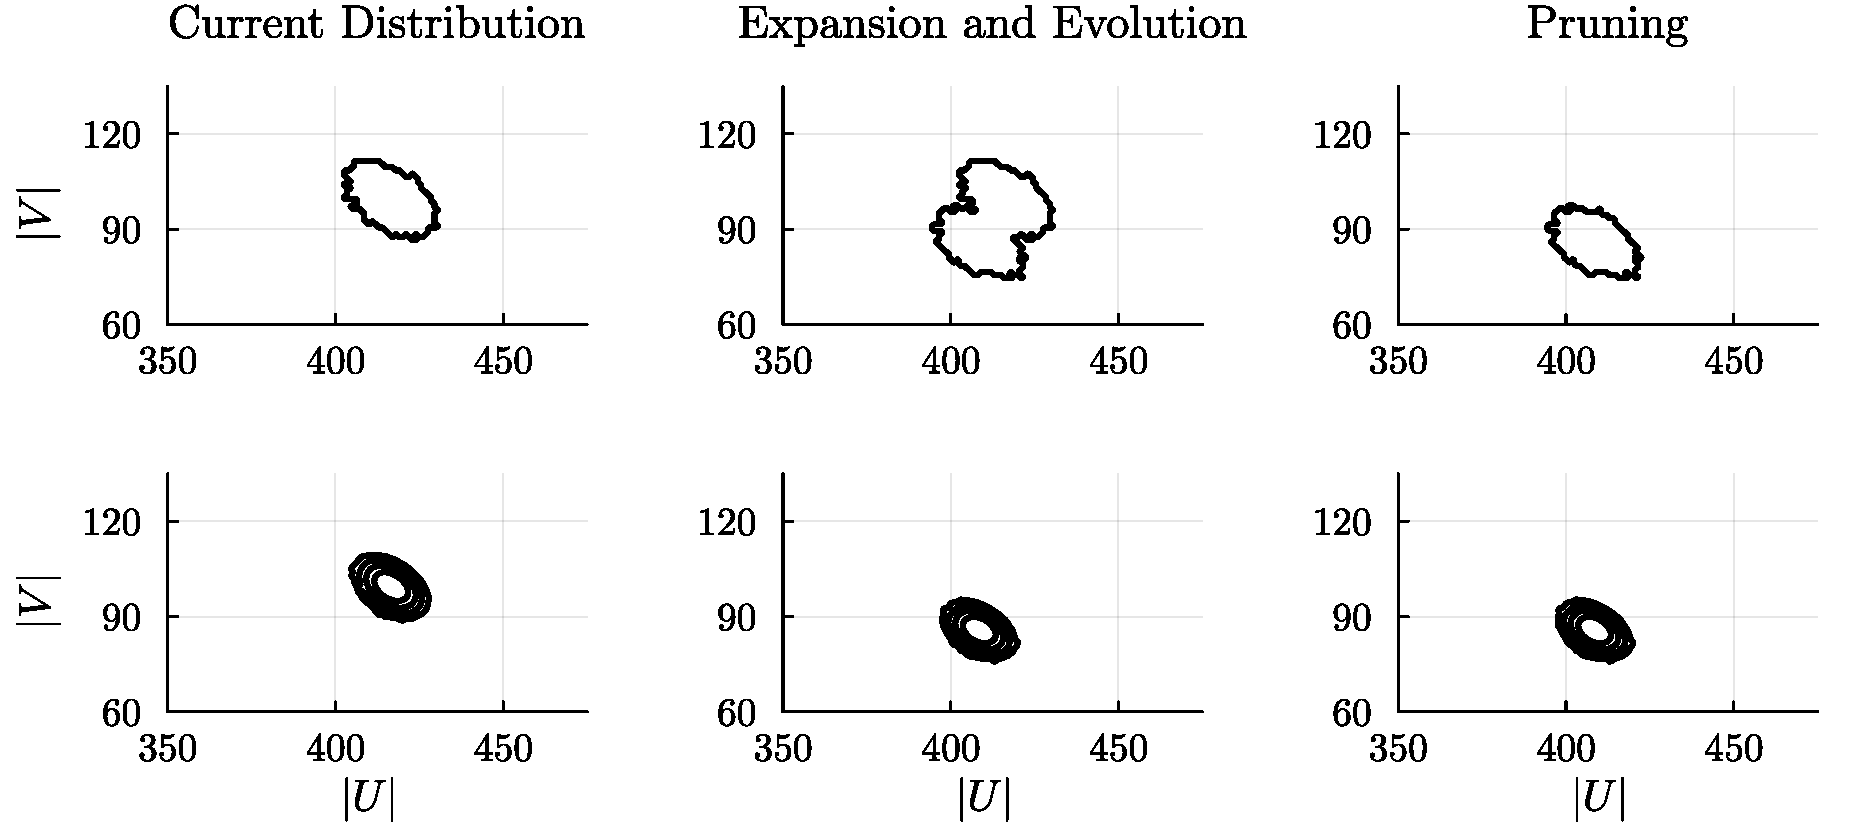
\includegraphics[width=\linewidth]{lv_grid.pdf}
    \caption{Visualization of the adaptive FSP procedure (species $U$ and $V$) during a single time step in Algorithm~\ref{alg:fsp-naive}. The top row shows the truncation boundary during the expand, evolve, and prune phases, while the bottom row shows the corresponding probability contours.}
    \label{fig:adapt-FSP}
\end{figure}

For simulations over long time intervals, maintaining a single fixed projection space is generally impractical: the reachable state space grows combinatorially in time, quickly making a static truncation too large to store or inefficient to evolve. A natural approach is to partition the time domain $[0,T]$ into subintervals $[t_k,t_{k+1}]$ and solve a sequence of restricted CME problems, each posed on a projection space $\mathbf{X}_J^{(k)}$ tailored to the states that are relevant during that subinterval \cite{Wolf2010, Dinh_2020}.  
At each time step, the method initializes $\boldsymbol{p}_J^{(k)}(t_k)$ from the previous solution, expands $\mathbf{X}_J^{(k)}$ to include newly reachable states, evolves the distribution forward in time, and prunes states whose probabilities fall below a chosen tolerance.

\begin{algorithm}[H]
\caption{FSP with Time Stepping and State Space Control}
\label{alg:fsp-naive}
\begin{algorithmic}[1]
\REQUIRE initial state $x_0$, time range $[t_0,t_f]$, propensities $\{\alpha_k(x)\}$, stoichiometries $\{\nu_k\}$, step $\Delta t$
\STATE $t \gets t_0$, \; $J \gets \{x_0\}$, \; $\boldsymbol{p} \gets [1]$
\WHILE{$t < t_f$}
  \STATE \textbf{Expand:} add neighbors of $J$ reachable by one (or preset $r$) reactions
  \STATE \textbf{Assemble:} build $\mathbf{A}_{JJ}$ on $J$
  \STATE \textbf{Evolve:} $\boldsymbol{p} \gets \exp(\mathbf{A}_{JJ}\Delta t)\,\boldsymbol{p}$
  \STATE \textbf{Prune:} remove states with $p(x)$ below a heuristic threshold
  \STATE $t \gets \min\{t+\Delta t,\,t_f\}$
\ENDWHILE
\STATE \textbf{return} $(J,\boldsymbol{p})$ at $t_f$
\end{algorithmic}
\end{algorithm}

This \emph{sliding-window} approach provides a general template for adaptive FSP methods with dynamically evolving state spaces \cite{Dinh2016}. Many variants differ in how expansion and pruning are performed, but they all follow the same broad framework which is to enlarge the state space to capture new probability flow, evolve the distribution on the truncated generator, and prune regions that have become irrelevant. 
The remainder of this paper focuses on refining and analyzing the pruning and time step determination steps within this general adaptive FSP skeleton.


\begin{remark}[Stiffness and multiscale challenges in adaptive FSP]
\label{rem:stiffness-challenges}
Adaptive FSP methods must grapple with stiffness that arises when the generator $\mathbf{A}$ exhibits a wide separation of timescales across the state space, a characteristic of many biochemical reaction networks. This stiffness manifests in two coupled ways. First, \textit{spatial stiffness} emerges through connectivity bottlenecks. As illustrated in Figure~\ref{fig:bottleneck}, a bridge state $s_b$ with negligible probability but large exit rate $w(s_b) := \sum_{k=1}^M \alpha_k(s_b)$ (defined formally in Definition~\ref{def:flux}) creates a fast pathway between slow metastable regions, and pruning $s_b$ based on probability alone severs this connection, rendering the generator reducible and trapping probability mass in isolated components. Second, stiffness also manifests itself temporally. When probability rapidly redistributes during transient phases, the total flux $\Phi_{\mathrm{total}}(t) = \sum_{\boldsymbol{x}} p(\boldsymbol{x},t) w(\boldsymbol{x})$ becomes large and requires small steps $\Delta t$ for stability, while metastable slow periods with low flux permit large steps for efficiency (Figure~\ref{fig:temporal-stiffness}). These manifestations are coupled through the exit rates $w(\boldsymbol{x})$, which simultaneously create spatial bottlenecks and drive temporal flux variations. Our objective is to design pruning and time-stepping heuristics that jointly address both challenges, preserving network connectivity through flux-aware state selection while adapting $\Delta t$ to track the instantaneous activity level $\Phi_{\mathrm{total}}(t)$, thereby maintaining both structural integrity and computational tractability for robust multiscale simulation.

% Requires: \usepackage{subcaption}
\begin{figure}[ht!]
\centering

\begin{subfigure}[b]{0.46\textwidth}
\centering
\resizebox{\linewidth}{!}{%
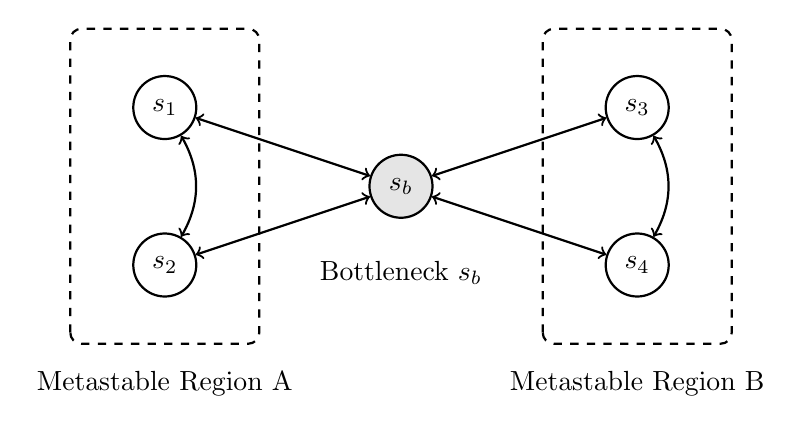
\begin{tikzpicture}[node distance=2.2cm, auto, thick,
  state/.style={circle, draw, minimum size=0.8cm}]
  \node[state] (A1) at (0,1) {$s_1$};
  \node[state] (A2) at (0,-1) {$s_2$};
  \node[state, fill=gray!20] (B) at (3,0) {$s_b$};
  \node[state] (C1) at (6,1) {$s_3$};
  \node[state] (C2) at (6,-1) {$s_4$};

  \path[<->, thick] (A1) edge[bend left] (A2);
  \path[<->, thick] (C1) edge[bend left] (C2);
  \path[<->, thick] (A1) edge (B);
  \path[<->, thick] (A2) edge (B);
  \path[<->, thick] (C1) edge (B);
  \path[<->, thick] (C2) edge (B);

  \draw[dashed, rounded corners] (-1.2,-2) rectangle (1.2,2);
  \draw[dashed, rounded corners] (4.8,-2) rectangle (7.2,2);

  \node at (0, -2.5) {Metastable Region A};
  \node at (6, -2.5) {Metastable Region B};
  \node at (3, -1.1) {Bottleneck $s_b$};
\end{tikzpicture}%
}
\caption{}
\label{fig:bottleneck}
\end{subfigure}
\hfill
\begin{subfigure}[b]{0.46\textwidth}
\centering
\resizebox{\linewidth}{!}{%
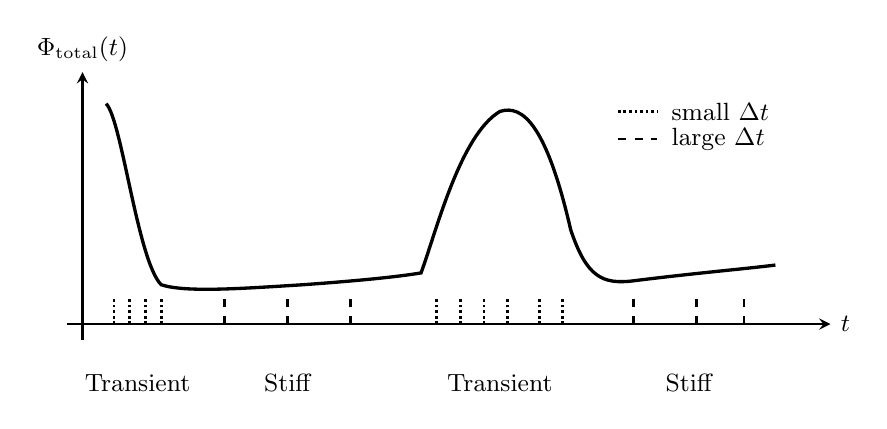
\begin{tikzpicture}[thick]
  % Axes
  \draw[->, >=stealth, thick] (-0.2,0) -- (9.5,0) node[right, font=\small] {$t$};
  \draw[->, >=stealth, thick] (0,-0.2) -- (0,3.2) node[above, font=\small] {$\Phi_{\text{total}}(t)$};
  % Curve with steeper transients and gently varying stiff regions
  \draw[line width=1.2pt]
    (0.3,2.8) .. controls (0.5,2.6) and (0.7,0.8) .. (1.0,0.5)
    .. controls (1.3,0.4) and (2.0,0.45) .. (2.8,0.5)
    .. controls (3.5,0.55) and (4.0,0.6) .. (4.3,0.65)
    .. controls (4.5,1.2) and (4.8,2.4) .. (5.3,2.7)
    .. controls (5.6,2.8) and (5.9,2.5) .. (6.2,1.2)
    .. controls (6.4,0.6) and (6.6,0.5) .. (7.0,0.55)
    .. controls (7.8,0.65) and (8.4,0.7) .. (8.8,0.75);
  % Small Δt ticks (transient regions)
  \foreach \x in {0.4,0.6,0.8,1.0,4.5,4.8,5.1,5.4,5.8,6.1}
    \draw[densely dotted, line width=1pt] (\x,0) -- (\x,0.35);
  % Large Δt ticks (stiff regions)
  \foreach \x in {1.8,2.6,3.4,7.0,7.8,8.4}
    \draw[dashed, line width=1pt] (\x,0) -- (\x,0.35);
  % Region labels
  \node[font=\small] at (0.7,-0.75) {Transient};
  \node[font=\small] at (2.6,-0.75) {Stiff};
  \node[font=\small] at (5.3,-0.75) {Transient};
  \node[font=\small] at (7.7,-0.75) {Stiff};
  % Legend
  \begin{scope}[shift={(6.8,2.7)}]
    \draw[densely dotted, line width=1pt] (0,0) -- (0.5,0);
    \node[right, font=\small] at (0.55,0) {small $\Delta t$};
    \draw[dashed, line width=1pt] (0,-0.35) -- (0.5,-0.35);
    \node[right, font=\small] at (0.55,-0.35) {large $\Delta t$};
  \end{scope}
\end{tikzpicture}%
}
\caption{}
\label{fig:temporal-stiffness}
\end{subfigure}
\caption{Illustration of stiffness in both spatial and temporal domains. (\subref{fig:bottleneck}) shows a bottleneck state $s_b$ that connects metastable regions, while (\subref{fig:temporal-stiffness}) shows alternating transient and stiff regimes reflected in the total flux $\Phi_{\text{total}}(t)$.}
\label{fig:stiffness-combined}
\end{figure}
\end{remark}

\section{Methodology: Flux-Based Adaptive FSP}
\label{sec:methodology}

This section introduces a state space adaptation approach that preserves network connectivity through flux-aware truncation. We first define and characterize probability flux as a connectivity measure, argue that naive probability-based pruning can destroy essential pathways, then construct an algorithm that maintains structural integrity of the state-space graph while controlling computational cost.

\begin{definition}[Outgoing probability flux]
\label{def:flux}
Let $w(\boldsymbol{x}) := \sum_{k=1}^M \alpha_k(\boldsymbol{x}) = -\mathbf{A}_{\boldsymbol{x},\boldsymbol{x}}$ denote the total exit rate from state $\boldsymbol{x}$. The \textit{outgoing probability flux} from state $\boldsymbol{x}$ at time $t$ is
\begin{equation}
\Phi(\boldsymbol{x},t) := p(\boldsymbol{x},t) \cdot w(\boldsymbol{x}).
\end{equation}
\end{definition}

The flux $\Phi(\boldsymbol{x},t)$ measures the instantaneous rate at which probability mass exits state $\boldsymbol{x}$. For small $\Delta t > 0$, approximately $\Phi(\boldsymbol{x},t) \cdot \Delta t$ units of probability mass leave $\boldsymbol{x}$ during the interval $[t, t+\Delta t]$. Crucially, states with large exit rates $w(\boldsymbol{x})$ but low probabilities $p(\boldsymbol{x},t)$ can maintain significant flux, acting as critical connections for probability flow between regions of state space despite being rarely occupied.

\begin{definition}[Total system flux]
The total probability flux of the system at time $t$ over state set $J$ is
\begin{equation}
\Phi_{\mathrm{total}}(J,t) := \sum_{\boldsymbol{x} \in J} \Phi(\boldsymbol{x},t) = \sum_{\boldsymbol{x} \in J} p(\boldsymbol{x},t) \cdot w(\boldsymbol{x}).
\end{equation}
\end{definition}

\begin{proposition}[Total flux properties]
\label{prop:total-flux}
For the full state space $\mathcal{X}$ and any time $t \geq 0$, the total system flux satisfies
\begin{equation}
\Phi_{\mathrm{total}}(\mathcal{X},t) = \sum_{\boldsymbol{x} \in \mathcal{X}} p(\boldsymbol{x},t) \cdot w(\boldsymbol{x}) = -\boldsymbol{p}(t)^\top \mathrm{diag}(\mathbf{A}).
\end{equation}
Since $\sum_{\boldsymbol{x}} p(\boldsymbol{x},t) = 1$ for all $t$, the total flux represents a weighted average of exit rates across the state space. For reaction networks with mass-action or similar kinetics where exit rates grow at most polynomially with state values, $\Phi_{\mathrm{total}}(\mathcal{X},t)$ remains bounded on compact time intervals and tracks the instantaneous activity level of the system.
\end{proposition}

\begin{proof}
By definition of the generator matrix,
\begin{align}
\Phi_{\mathrm{total}}(\mathcal{X},t) &= \sum_{\boldsymbol{x} \in \mathcal{X}} p(\boldsymbol{x},t) \cdot (-\mathbf{A}_{\boldsymbol{x},\boldsymbol{x}}) = -\boldsymbol{p}(t)^\top \mathrm{diag}(\mathbf{A}).
\end{align}
Since the diagonal entries $\mathbf{A}_{\boldsymbol{x},\boldsymbol{x}} = -\sum_{k=1}^M \alpha_k(\boldsymbol{x})$ depend only on the reaction network structure and state $\boldsymbol{x}$, the total flux evolves with the probability distribution. 
\end{proof}

\subsection{Flux and Network Connectivity}
\label{sec:flux-connectivity}

Having defined flux, we briefly review how it connects to the structural properties governing long-time behavior. This connection motivates our pruning rule, though the error bounds in Section~\ref{sec:theory} will take a more direct approach based on system fluxes. A generator $\mathbf{A}$ on a finite state space $J$ is \textit{irreducible} if the corresponding state-space graph is strongly connected. Equivalently (with our column convention, where $A_{x,y}>0$ is a transition $y\!\to\!x$), there is no nontrivial partition $J=J_1\cup J_2$ with $J_1\cap J_2=\emptyset$ such that $A_{J_1,J_2}=0$ (no transitions from $J_2$ into $J_1$). Irreducibility ensures that the chain can reach any state from any other in finite expected time and implies a unique stationary distribution $\boldsymbol{\pi}\gg 0$ for the finite continuous time Markov chains. The spectral gap
\[
\lambda := \min\{\operatorname{Re}(-\lambda_k(\mathbf{A})):\lambda_k(\mathbf{A})\neq 0\} > 0
\]
governs exponential convergence to stationarity (e.g., in $\pi$-weighted norms), i.e., $\|\boldsymbol{p}(t)-\boldsymbol{\pi}\|\le C e^{-\lambda t}$. The connection between flux and connectivity is formalized through Cheeger's inequality for continuous-time Markov chains \cite{Diaconis1991,63529}. Define the \textit{conductance} of a subset $S \subset J$ as
\begin{equation}
\Psi(S) := \frac{\sum_{\boldsymbol{x} \in S}\sum_{\boldsymbol{y} \in J \setminus S} \pi(\boldsymbol{x}) \mathbf{A}_{\boldsymbol{y},\boldsymbol{x}}}{\min\{\pi(S), \pi(J\setminus S)\}},
\label{eq:cheeger}
\end{equation}
where $\pi(S) := \sum_{\boldsymbol{x} \in S} \pi(\boldsymbol{x})$. Let $\Psi_* := \min_{S: 0 < \pi(S) \leq 1/2} \Psi(S)$ denote the minimum conductance, which quantifies the flux across the most restrictive bottleneck in the state-space graph. The numerator of the conductance $\Psi(S)$ is precisely the stationary flux across the cut $S$. Our flux-based pruning rule protects states with high instantaneous flux $\Phi(x,t) = p(x,t) w(x)$, which at stationarity coincides with the contributions to this numerator. Thus, removing high-flux states risks collapsing the conductance of critical cuts, degrading $\Psi_*$ and hence the spectral gap $\lambda$ via \eqref{eq:cheeger}. Cheeger's inequality establishes the two-sided bound
\begin{equation}
\label{eq:cheeger1}
\frac{\Psi_*^2}{2} \leq \lambda \leq 2\Psi_*,
\end{equation}
linking the spectral gap to the minimum conductance. Removing high-flux bridge states reduces $\Psi_*$, which by \eqref{eq:cheeger1} degrades $\lambda$ and slows convergence. In the extreme case where all paths between two regions are severed, $\Psi_*=0$ and irreducibility is lost entirely. The key insight is that a bridge state can have $p(\boldsymbol{x}_b,t)\ll 1$ yet large flux $\Phi(\boldsymbol{x}_b,t)=p(\boldsymbol{x}_b,t)\,w(\boldsymbol{x}_b)$ when its exit rate $w(\boldsymbol{x}_b)=-A_{\boldsymbol{x}_b,\boldsymbol{x}_b}$ is large. In an adaptive FSP approach we replace one very large sparse generator by a sequence of smaller truncated generators. To keep long-time behavior stable across this sequence, we want the spectral gap to remain nearly invariant under truncation. This means we must avoid pruning states whose removal collapses the gap. Flux provides a concrete measure for identifying high-flux bridge states that should not be truncated.

\subsubsection{Flux-Aware Truncation Algorithm}

We propose a two-stage pruning approach that combines probability-based candidate selection with flux-based protection. The algorithm identifies states for potential removal using a quantile threshold, then protects low-probability states that carry significant probability flow.

\begin{algorithm}[H]
\caption{Flux-Preserving Pruning}
\label{alg:flux-prune}
\begin{algorithmic}[1]
\REQUIRE Active set $\mathcal{S}$, probability vector $\boldsymbol{p}$, generator $\mathbf{A}$, quantile tolerance $\alpha \in (0,1)$, flux tolerance $\epsilon_{\mathrm{flux}} > 0$
\ENSURE Updated set $\mathcal{S}_{\mathrm{new}}$ and renormalized probability $\boldsymbol{p}_{\mathrm{new}}$
\STATE
\STATE \textit{Stage 1: Candidate Selection}
\STATE Sort states $\boldsymbol{x} \in \mathcal{S}$ in ascending order of $p(\boldsymbol{x}, t)$
\STATE Define candidate set $\mathcal{C} \subseteq \mathcal{S}$ as the minimal set satisfying
\begin{equation}
\sum_{\boldsymbol{x} \in \mathcal{C}} p(\boldsymbol{x}, t) \leq \alpha \quad \text{and} \quad p(\boldsymbol{x}, t) \leq p(\boldsymbol{y}, t) \; \forall \boldsymbol{x} \in \mathcal{C}, \boldsymbol{y} \in \mathcal{S} \setminus \mathcal{C}
\end{equation}
\STATE \textit{Stage 2: Flux-Based Protection}
\FOR{each $\boldsymbol{x} \in \mathcal{S}$}
    \STATE Compute exit rate: $w(\boldsymbol{x}) = -\mathbf{A}_{\boldsymbol{x},\boldsymbol{x}}$
    \STATE Compute flux: $\Phi(\boldsymbol{x}, t) = p(\boldsymbol{x}, t) \cdot w(\boldsymbol{x})$
\ENDFOR
\STATE Compute total flux: $\Phi_{\mathrm{total}} = \sum_{\boldsymbol{x} \in \mathcal{S}} \Phi(\boldsymbol{x}, t)$
\STATE Set flux threshold: $\Phi_{\mathrm{thr}} = \epsilon_{\mathrm{flux}} \cdot \Phi_{\mathrm{total}}$
\STATE Define protected set: $\mathcal{P} = \{\boldsymbol{x} \in \mathcal{C} : \Phi(\boldsymbol{x}, t) \geq \Phi_{\mathrm{thr}}\}$
\STATE Define pruning set: $\mathcal{S}_{\mathrm{prune}} = \mathcal{C} \setminus \mathcal{P}$
\STATE
\STATE \textit{Stage 3: Update and Renormalization}
\STATE $\mathcal{S}_{\mathrm{new}} \gets \mathcal{S} \setminus \mathcal{S}_{\mathrm{prune}}$
\STATE $\boldsymbol{p}_{\mathrm{new}} \gets \boldsymbol{p}|_{\mathcal{S}_{\mathrm{new}}} / \|\boldsymbol{p}|_{\mathcal{S}_{\mathrm{new}}}\|_1$ \quad (restrict and renormalize)
\RETURN $\mathcal{S}_{\mathrm{new}}, \boldsymbol{p}_{\mathrm{new}}$
\end{algorithmic}
\end{algorithm}

Stage 1 identifies low-probability candidate states for removal based on the quantile threshold $\alpha$. Without this candidate selection, the method would need to evaluate flux for every state at every pruning step, incurring unnecessary computational cost when most high-probability states are never at risk of removal. The quantile filter focuses computational effort on the tail of the distribution where pruning decisions are nontrivial. Stage 2 protects states in $\mathcal{C}$ that carry significant flux relative to total system flux. Consider a bottleneck state $s_b$ connecting metastable regions as seen in Figure~\ref{fig:bottleneck}. Such states transmit substantial probability flow between regions despite low occupancy. Removing them degrades conductance, shrinks the spectral gap, and harms mixing. The flux tolerance $\epsilon_{\mathrm{flux}}$ controls the trade-off between compression and connectivity preservation. Stage 3 removes unprotected candidates and renormalizes the probability distribution to maintain unit total mass.


\subsection{Adaptive Time Stepping}
We now address the temporal aspect of stiffness discussed in Remark~\ref{rem:stiffness-challenges}. The time step must adapt to the system's instantaneous activity level to maintain both stability and efficiency. Our approach is inspired by tau-leaping methods for stochastic simulation \cite{Gillespie2001, CAO20083472}, which choose time steps based on propensity bounds to limit the expected number of events per step. The total system flux $\Phi_{\mathrm{total}}(\mathcal{S}_n, t_n)$ plays a role analogous to stiffness indicators in stiff ODE theory: quantities based on logarithmic norms of the Jacobian define a natural timescale for the fastest active processes \cite{Soderlind2015-ai}, and the total flux plays the same role for the truncated CME system. Since the rate of probability leaving the truncated domain is bounded above by $\Phi_{\mathrm{total}}$ (Corollary~\ref{cor:flux-timestep}), we choose the time step as
\begin{equation}
\label{eq:flux-timestep}
\Delta t_n = \frac{\epsilon_{\Delta t}}{\Phi_{\mathrm{total}}(\mathcal{S}_n, t_n)},
\end{equation}
where $\epsilon_{\Delta t}$ is a dimensionless tolerance parameter. This rule ensures that $\Delta t_n \cdot \Phi_{\mathrm{total}}(t_n) = \epsilon_{\Delta t}$, bounding the total probability mass that can cross the truncation boundary during the step. The formal justification follows from the local error analysis in Section~\ref{sec:theory}.


\subsection{Master Equation Matrix Construction}
\label{sec:matrix_construction}

The generator matrix $\mathbf{A}(t)$ must be constructed at each adaptive time step as the state space evolves. We employ a forward enumeration approach that exploits the sparse reaction connectivity structure to build the matrix efficiently. For a given state set $\mathcal{S}$ with $n = |\mathcal{S}|$ states and $R$ reaction channels, we construct $\mathbf{A}$ column by column. For each state $x \in \mathcal{S}$ and reaction $k$ with stoichiometry $\boldsymbol{\nu}_k$, we compute the destination state $y = x + \boldsymbol{\nu}_k$. If $y \in \mathcal{S}$, we evaluate the propensity $\alpha_k(x)$ and place it at position $(i_y, i_x)$ in the matrix, where $i_y$ and $i_x$ are the indices of states $y$ and $x$ in $\mathcal{S}$. We accumulate these off-diagonal entries to compute the column sum, then set the diagonal entry to the negative of this sum to ensure the generator property (zero column sums).

\begin{algorithm}[H]
\caption{Forward Enumeration Matrix Construction}
\label{alg:matrix_construction}
\begin{algorithmic}[1]
\REQUIRE State set $\mathcal{S}$, reaction model with stoichiometries $\{\boldsymbol{\nu}_k\}$ and propensities $\{\alpha_k\}$
\ENSURE Generator matrix $\mathbf{A}$
\STATE Initialize sparse matrix arrays: $I \leftarrow []$, $J \leftarrow []$, $V \leftarrow []$
\STATE Create index mapping: $\texttt{state\_id}: \mathcal{S} \rightarrow \{1, \ldots, |\mathcal{S}|\}$
\FOR{each state $x \in \mathcal{S}$ with index $j$}
    \STATE $\text{col\_sum} \leftarrow 0$
    \FOR{each reaction $k$ with stoichiometry $\boldsymbol{\nu}_k$}
        \STATE $y \leftarrow x + \boldsymbol{\nu}_k$
        \IF{$y \in \mathcal{S}$}
            \STATE $\alpha \leftarrow \texttt{propensity}_k(x)$
            \IF{$\alpha > 0$}
                \STATE $i \leftarrow \texttt{state\_id}[y]$
                \STATE Append $(i, j, \alpha)$ to sparse arrays
                \STATE $\text{col\_sum} \leftarrow \text{col\_sum} + \alpha$
            \ENDIF
        \ENDIF
    \ENDFOR
    \IF{$\text{col\_sum} > 0$}
        \STATE Append $(j, j, -\text{col\_sum})$ to sparse arrays \COMMENT{Diagonal entry}
    \ENDIF
\ENDFOR
\STATE $\mathbf{A} \leftarrow \texttt{sparse}(I, J, V, |\mathcal{S}|, |\mathcal{S}|)$
\RETURN $\mathbf{A}$
\end{algorithmic}
\end{algorithm}

The computational complexity is $O(|\mathcal{S}| \cdot R)$ for iterating through states and reactions. This exploits the sparse structure of the reaction graph as each state connects to at most $R$ other states through direct chemical transformations, avoiding the $O(|\mathcal{S}|^2)$ cost of checking all possible state pairs. For typical chemical reaction networks with $R \ll |\mathcal{S}|$, this forward enumeration approach yields substantial performance improvements over standard backward expansion methods.

\begin{remark}
Algorithm~\ref{alg:matrix_construction} directly constructs the compressed generator $\widetilde{\mathbf{A}}_{JJ}$ of~\eqref{eq:compressed-generator}, not the truncated generator $\mathbf{A}_{JJ}$. For each source state $x \in J$ and reaction $k$, a propensity $\alpha_k(x)$ contributes to the off-diagonal entry at row $y = x + \boldsymbol{\nu}_k$ only if $y \in J$; the diagonal is then set to the negative of this partial column sum. Transitions whose destination falls outside $J$ are excluded from both the off-diagonal and the diagonal, so the column sums are exactly zero by construction. This is precisely the defining property of $\widetilde{\mathbf{A}}_{JJ}$ (Proposition~\ref{prop:compressed-generator}, property~1), and consequently the evolution step $\boldsymbol{p} \gets e^{\widetilde{\mathbf{A}}_{JJ}\Delta t}\boldsymbol{p}$ conserves probability: $\boldsymbol{1}^\top\boldsymbol{p}$ is invariant under time evolution.

The renormalization $\boldsymbol{p} \gets \boldsymbol{p}/\|\boldsymbol{p}\|_1$ that appears in Algorithm~\ref{alg:flux-prune} (Stage~3) serves a different purpose: it compensates for the probability mass discarded when states are removed during pruning, not for any leakage from the generator. This pruned mass is at most $\alpha$ by the quantile selection in Stage~1. Thus the theoretical error analysis, which is formulated in terms of the compressed generator $\widetilde{\mathbf{A}}_{JJ}$, applies directly to the implemented algorithm without any additional approximation gap.
\end{remark}

\subsection{Full Algorithm}
\label{sec:full-algorithm}
This section presents the complete flux-adaptive FSP method integrating the components developed above including boundary expansion, forward enumeration matrix construction (Algorithm~\ref{alg:matrix_construction}), flux-based adaptive time stepping (Eq.~\eqref{eq:flux-timestep}), and connectivity-preserving pruning (Algorithm~\ref{alg:flux-prune}). The algorithm maintains a dynamically adapted state space $\mathcal{S}$ that expands to capture emerging probability mass and contracts via flux-aware pruning to control computational cost while preserving network connectivity.

\begin{algorithm}[H]
\caption{Flux-Adaptive FSP}
\label{alg:fsp-flux-adaptive}
\begin{algorithmic}[1]
\REQUIRE initial state $x_0$, time range $[t_0,t_f]$, propensities $\{\alpha_k(x)\}$, stoichiometries $\{\nu_k\}$, quantile tolerance $\alpha$, flux tolerance $\epsilon_{\mathrm{flux}}$, time step tolerance $\epsilon_{\Delta t}$
\STATE $t \gets t_0$, \; $\mathcal{S} \gets \{x_0\}$, \; $\boldsymbol{p} \gets [1]$, \; $\mathbf{A} \gets$ initial generator
\WHILE{$t < t_f$}
  \STATE \textbf{Expand:} $\mathcal{S}_{\text{new}} \gets \mathcal{S} \cup \partial \mathcal{S}$ (expand state space)
  \STATE \textbf{Construct:} $\mathbf{A}_{\text{new}} \gets$ forward enumeration (Algorithm~\ref{alg:matrix_construction})
  \STATE \textbf{Adapt step:} Compute $\Phi_{\mathrm{total}} = \sum_{x \in \mathcal{S}_{\text{new}}} p(x,t) \cdot w(x)$ and set $\Delta t = \epsilon_{\Delta t}/\Phi_{\mathrm{total}}$ (Eq.~\eqref{eq:flux-timestep})
  \STATE \textbf{Evolve:} $\boldsymbol{p} \gets \exp(\mathbf{A}_{\text{new}}\Delta t)\,\boldsymbol{p}$
  \STATE \textbf{Prune:} $(\mathcal{S}_{\text{pruned}}, \boldsymbol{p}_{\text{pruned}}) \gets$ flux-preserving pruning (Algorithm~\ref{alg:flux-prune}) with parameters $\alpha, \epsilon_{\mathrm{flux}}$
  \STATE $\mathcal{S} \gets \mathcal{S}_{\text{pruned}}$, \; $\boldsymbol{p} \gets \boldsymbol{p}_{\text{pruned}}$, \; $\mathbf{A} \gets \mathbf{A}_{\text{new}}|_{\mathcal{S}_{\text{pruned}}}$
  \STATE $t \gets \min\{t+\Delta t,\,t_f\}$
\ENDWHILE
\STATE \textbf{return} $(\mathcal{S},\boldsymbol{p})$ at $t_f$
\end{algorithmic}
\end{algorithm}



The computational bottleneck is the matrix exponential action $\exp(\mathbf{A}_{\text{new}}\Delta t)\boldsymbol{p}$ in the evolution step. We employ Krylov subspace methods via the EXPOKIT package \cite{Sidje1998}, which computes matrix exponential actions without forming the full exponential matrix. For a sparse generator $\mathbf{A}$ of dimension $n = |\mathcal{S}|$ with
$\mathrm{nnz}(\mathbf{A}) = O(n)$, EXPOKIT's Krylov--Arnoldi routine for
computing $e^{t\mathbf{A}} v$ has per-step cost
\[
  O\bigl(m\,\mathrm{nnz}(\mathbf{A}) + m^2 n\bigr) = O(m^2 n),
\]
where $m \ll n$ is the Krylov subspace dimension. In our setting, the
expansion and pruning operations scale as $O(nR)$, and constructing
$\mathbf{A}$ by forward enumeration also costs $O(nR)$, where $R$ is the
number of reactions. Since $m$ and $R$ are small constants independent of
$n$, the total per-step cost is effectively linear in the state-space size,
making simulations with $10^4$--$10^5$ states computationally tractable.


\section{Error Analysis}
\label{sec:theory}

We derive local and global error bounds for the adaptive FSP method based on probability fluxes across the truncation boundary. Let $\mathcal{X}$ denote the full state space and $J \subset \mathcal{X}$ be a finite active set. Define the complement $J' := \mathcal{X} \setminus J$ with $J \cap J' = \emptyset$ and $J \cup J' = \mathcal{X}$. The generator matrix admits a natural block decomposition:

\begin{equation}
\label{eq:block-partition}
\mathbf{A}=
\begin{pmatrix}
\mathbf{A}_{JJ} & \mathbf{A}_{JJ'}\\
\mathbf{A}_{J'J} & \mathbf{A}_{J'J'}
\end{pmatrix}, 
\qquad
\boldsymbol{p}(t)=
\begin{pmatrix}
\boldsymbol{p}_J(t)\\
\boldsymbol{p}_{J'}(t)
\end{pmatrix},
\end{equation}
Recall that under the column convention $\mathbf{A}_{ij} > 0$ represents a transition rate \emph{from} state $j$ \emph{to} state $i$. Accordingly, the block subscripts follow matrix index order (rows, columns): $\mathbf{A}_{JJ} \in \mathbb{R}^{|J| \times |J|}$ has rows and columns in $J$ and governs transitions within $J$; $\mathbf{A}_{J'J} \in \mathbb{R}^{|J'| \times |J|}$ has rows in $J'$ and columns in $J$, so its entries $(\mathbf{A}_{J'J})_{\boldsymbol{y}\boldsymbol{x}} = \mathbf{A}_{\boldsymbol{y}\boldsymbol{x}}$ for $\boldsymbol{y} \in J'$, $\boldsymbol{x} \in J$ describe transitions \emph{from} $J$ \emph{to} $J'$ (outflux); symmetrically, $\mathbf{A}_{JJ'} \in \mathbb{R}^{|J| \times |J'|}$ describes transitions \emph{from} $J'$ \emph{to} $J$ (influx). See Figure~\ref{fig:transitions}. The partitioned CME becomes:
\begin{equation}
\label{eq:partitioned-cme}
\frac{d}{dt}
\begin{pmatrix}
\boldsymbol{p}_J(t) \\
\boldsymbol{p}_{J'}(t)
\end{pmatrix}
=
\begin{pmatrix}
\mathbf{A}_{JJ} & \mathbf{A}_{JJ'}\\
\mathbf{A}_{J'J} & \mathbf{A}_{J'J'}
\end{pmatrix}
\begin{pmatrix}
\boldsymbol{p}_J(t) \\
\boldsymbol{p}_{J'}(t)
\end{pmatrix},
\end{equation}
where, 
\begin{equation}
\label{eq:row-sum-identities}
\mathbf{1}^\top \mathbf{A}_{JJ} = -\mathbf{1}^\top \mathbf{A}_{J'J}, \qquad \mathbf{1}^\top \mathbf{A}_{J'J'} = -\mathbf{1}^\top \mathbf{A}_{JJ'}.
\end{equation}
The column sum property of the generator $\mathbf{A}$ immediately yields the identities in Eq.~\eqref{eq:row-sum-identities}.
\begin{figure}[ht!]
    \centering
    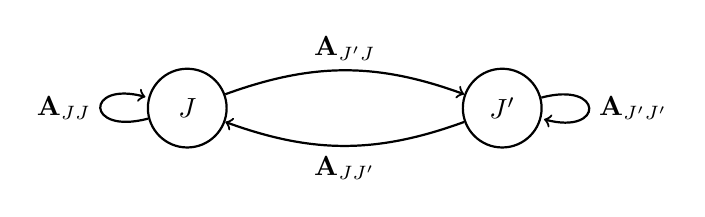
\begin{tikzpicture}[node distance=3cm, auto, thick]
    \tikzstyle{state} = [circle, draw, minimum size=1cm, text centered]
    \tikzstyle{transition} = [->, thick]
    \node[state] (S) at (0, 0) {$J$};
    \node[state] (R) at (4, 0) {$J'$};
    \path[transition, loop left] (S) edge node[left] {$\mathbf{A}_{JJ}$} (S);
    \path[transition, loop right] (R) edge node[right] {$\mathbf{A}_{J'J'}$} (R);
    \path[transition] (S) edge[bend left=20] node[above] {$\mathbf{A}_{J'J}$} (R);
    \path[transition] (R) edge[bend left=20] node[below] {$\mathbf{A}_{JJ'}$} (S);
    \end{tikzpicture}
    \caption{Partitioned master equation transitions between the active set $J$ and its complement $J'$.}
    \label{fig:transitions}
\end{figure}


We define the boundary flux rates as
\begin{equation}
\label{eq:flux-defs}
\Phi_{\mathrm{out}}(t) := \mathbf{1}^\top \mathbf{A}_{J'J}\boldsymbol{p}_J(t), \qquad \Phi_{\mathrm{in}}(t) := \mathbf{1}^\top \mathbf{A}_{JJ'}\boldsymbol{p}_{J'}(t),
\end{equation}
where $\Phi_{\mathrm{out}}(t)$ is the total probability mass per unit time flowing from $J$ to $J'$ (the block $\mathbf{A}_{J'J}$ acts on $\boldsymbol{p}_J$ since its columns are indexed by $J$ and its entries give rates \emph{into} $J'$), and $\Phi_{\mathrm{in}}(t)$ is the mass flowing from $J'$ to $J$ (the block $\mathbf{A}_{JJ'}$ acts on $\boldsymbol{p}_{J'}$ since its columns are indexed by $J'$ and its entries give rates \emph{into} $J$). Both quantities are non-negative. The original FSP approach defines an absorbing sink state that collapses the complement of the truncated set. Following the block formulation, it is equivalent to the \textit{compressed generator} formed by adding the outgoing probability flux back to the diagonal elements:
\begin{equation}
\label{eq:compressed-generator}
\widetilde{\mathbf{A}}_{JJ} := \mathbf{A}_{JJ} + \diag(\mathbf{1}^\top \mathbf{A}_{J'J}),
\end{equation}
where $\operatorname{diag}(.)$ embeds a vector into the diagonal of a matrix. This operation ensures that any probability mass that would have left $J$ (as governed by $\mathbf{A}_{J'J}$) is instantaneously reflected back to its state of origin, creating a reflecting boundary condition.

\begin{proposition}[Compressed generator properties]
\label{prop:compressed-generator}
The compressed generator $\widetilde{\mathbf{A}}_{JJ}$ satisfies:
\begin{enumerate}
\item $\mathbf{1}^\top \widetilde{\mathbf{A}}_{JJ} = \mathbf{0}^\top$ (zero column sums, hence mass conservation),
\item $\widetilde{A}_{\boldsymbol{x}\boldsymbol{y}} \geq 0$ for $\boldsymbol{x} \neq \boldsymbol{y}$ (non-negative off-diagonals),
\item $\widetilde{A}_{\boldsymbol{x}\boldsymbol{x}} \leq 0$ for all $\boldsymbol{x}$ (non-positive diagonal),
\item $e^{t\widetilde{\mathbf{A}}_{JJ}} \geq 0$ and $\|e^{t\widetilde{\mathbf{A}}_{JJ}}\|_{1 \to 1} = 1$ for all $t \geq 0$ (generates a positive stochastic semigroup).
\end{enumerate}
\end{proposition}

\begin{proof}
Properties (1)-(3) follow directly from the construction of $\widetilde{\mathbf{A}}_{JJ}$. For property (1), using Eq.~\eqref{eq:row-sum-identities} and $\mathbf{1}^\top \diag(\boldsymbol{v}) = \boldsymbol{v}^\top$,
\begin{align*}
\mathbf{1}^\top \widetilde{\mathbf{A}}_{JJ} = \mathbf{1}^\top \mathbf{A}_{JJ} + \mathbf{1}^\top \mathbf{A}_{J'J} = \mathbf{0}^\top.
\end{align*}
Property (2) holds because off-diagonal entries of $\widetilde{\mathbf{A}}_{JJ}$ equal those of $\mathbf{A}_{JJ}$, which are non-negative. For property (3), the diagonal entries are $\widetilde{A}_{xx} = A_{xx} + \sum_{y \in J'} A_{yx} = - \sum_{y \in J, y \neq x} A_{yx} \leq 0$. For property (4), we first establish the norm bound, then positivity. For any $\boldsymbol{p}(0) \geq \mathbf{0}$ with $\|\boldsymbol{p}(0)\|_1 = 1$, the solution $\boldsymbol{p}(t) = e^{t\widetilde{\mathbf{A}}_{JJ}}\boldsymbol{p}(0)$ satisfies
\begin{equation}
\frac{d}{dt}\|\boldsymbol{p}(t)\|_1 = \mathbf{1}^\top \frac{d\boldsymbol{p}}{dt} = \mathbf{1}^\top \widetilde{\mathbf{A}}_{JJ}\boldsymbol{p}(t) = (\mathbf{1}^\top \widetilde{\mathbf{A}}_{JJ})\boldsymbol{p}(t) = 0,
\end{equation}
by property (1). Therefore, $\|\boldsymbol{p}(t)\|_1 = \|\boldsymbol{p}(0)\|_1 = 1$ for all $t \geq 0$. Taking the supremum over all initial conditions yields $\|e^{t\widetilde{\mathbf{A}}_{JJ}}\|_{1 \to 1} = 1$. Next, we prove positivity: by properties (2)-(3), choose $\alpha \geq \max_{\boldsymbol{x}} |\widetilde{A}_{\boldsymbol{x}\boldsymbol{x}}|$ large enough that $\mathbf{B} := \widetilde{\mathbf{A}}_{JJ} + \alpha I$ has all non-negative entries. Then
\begin{align*}
e^{t\widetilde{\mathbf{A}}_{JJ}} &= e^{t(\mathbf{B} - \alpha I)} \\
                        &= e^{-\alpha t} e^{t\mathbf{B}} \\
                        &= e^{-\alpha t} \lim_{n \to \infty} \left(I + \frac{t}{n}\mathbf{B}\right)^n.
\end{align*}

Since $\mathbf{B} \geq 0$, each factor $I + \frac{t}{n}\mathbf{B} \geq 0$ for $t \geq 0$ and $n$ sufficiently large. Non-negative matrices are closed under multiplication, so $(I + \frac{t}{n}\mathbf{B})^n \geq 0$ for all $n$. Taking the limit and multiplying by the positive scalar $e^{-\alpha t} > 0$, we can conclude that $e^{t\widetilde{\mathbf{A}}_{JJ}} \geq 0$
\end{proof}
We now establish the contraction property for the truncated generator $\mathbf{A}_{JJ}$, which is needed for the local and global error bounds.

\begin{corollary}[Truncated generator contraction]
\label{cor:truncated-contraction}
The truncated generator $\mathbf{A}_{JJ}$ with non-positive column sums generates a positive contraction semigroup satisfying $e^{t\mathbf{A}_{JJ}} \geq 0$ and $\|e^{t\mathbf{A}_{JJ}}\|_{1 \to 1} \le 1$ for all $t \ge 0$.
\end{corollary}

\begin{proof}
For the norm bound, consider any $\boldsymbol{p}(0) \geq \mathbf{0}$ with $\|\boldsymbol{p}(0)\|_1 = 1$. Since $\mathbf{1}^\top \mathbf{A}_{JJ} \leq \mathbf{0}^\top$, we have
\begin{equation}
\frac{d}{dt}\|\boldsymbol{p}(t)\|_1 = \mathbf{1}^\top \mathbf{A}_{JJ}\boldsymbol{p}(t) = (\mathbf{1}^\top \mathbf{A}_{JJ})\boldsymbol{p}(t) \leq 0,
\end{equation}
which gives $\|e^{t\mathbf{A}_{JJ}}\|_{1 \to 1} \leq 1$. Positivity follows by the same shifting argument as in Proposition~\ref{prop:compressed-generator}.
\end{proof}

\begin{remark}[Infinite-dimensional extension]
\label{rem:infinite-dimensional}
The arguments in Proposition~\ref{prop:compressed-generator} and Corollary~\ref{cor:truncated-contraction} extend to the full CME on infinite state space $\mathcal{X}$ via the Hille-Yosida theorem~\cite{Ethier1986,pazy_1983}. In the infinite-dimensional setting, the operator $\mathbf{A}$ is unbounded on $\ell^1(\mathcal{X})$, requiring verification that $\mathbf{A}$ is closed with dense domain $D(\mathbf{A})$ and that the resolvent bounds $\|(\lambda I - \mathbf{A})^{-1}\|_{1 \to 1} \leq 1/\lambda$ hold for all $\lambda > 0$. These conditions guarantee that $\mathbf{A}$ generates a strongly continuous contraction semigroup. In our finite-dimensional truncation to $J$, all operators are automatically bounded and closed with domain equal to the entire space.
\end{remark}



\subsection{Local Error}

We decompose the local error into model error from state space truncation and time-stepping error from numerical approximation.

\subsubsection{Model Error from State Space Truncation}

Consider the dynamics on $J$ starting from the true state $\boldsymbol{p}_J(t_n)$. The true restricted dynamics satisfy

\begin{equation}
\label{eq:true-restricted}
\frac{d}{dt} \boldsymbol{p}_J(t) = \mathbf{A}_{JJ}\boldsymbol{p}_J(t) + \mathbf{A}_{JJ'}\boldsymbol{p}_{J'}(t),
\end{equation}
while the compressed dynamics evolve according to
\begin{equation}
\label{eq:compressed-dynamics-exact}
\frac{d}{dt} \widehat{\boldsymbol{p}}_J(t) = \widetilde{\mathbf{A}}_{JJ}\widehat{\boldsymbol{p}}_J(t).
\end{equation}
Define the local model error $\boldsymbol{\varepsilon}(t) := \boldsymbol{p}_J(t) - \widehat{\boldsymbol{p}}_J(t)$ with $\boldsymbol{\varepsilon}(t_n) = \mathbf{0}$.

\begin{theorem}[Local model error bound]
\label{thm:local-model-error}
Over a single time step $[t_n, t_{n+1}]$, the local model error satisfies
\begin{equation}
\|\boldsymbol{\varepsilon}(t_{n+1})\|_1 \leq \int_{t_n}^{t_{n+1}} (\Phi_{\mathrm{in}}(s) + \Phi_{\mathrm{out}}(s)) \; ds.
\end{equation}
where $\Phi_{\mathrm{in}}$ and $\Phi_{\mathrm{out}}$ are boundary fluxes entering and leaving the truncation boundary respectively (Eq.~\eqref{eq:flux-defs}).
\end{theorem}

\begin{proof}
Subtracting Eq.~\eqref{eq:compressed-dynamics-exact} from Eq.~\eqref{eq:true-restricted} gives the following inhomogeneous equation,
\begin{align*}
\frac{d}{dt}\boldsymbol{\varepsilon}(t) &= \mathbf{A}_{JJ}\boldsymbol{\varepsilon}(t) + \underbrace{\mathbf{A}_{JJ'}\boldsymbol{p}_{J'}(t) - \diag(\mathbf{1}^\top\mathbf{A}_{J'J})\widehat{\boldsymbol{p}}_J(t)}_{=: \boldsymbol{f}(t)}.
\end{align*}
The solution of the inhomogeneous ODE is given by,
\begin{align}
\boldsymbol{\varepsilon}(t_{n+1}) &= \int_{t_n}^{t_{n+1}} e^{(t_{n+1}-s)\mathbf{A}_{JJ}}\boldsymbol{f}(s) \, ds + e^{A_{JJ}}\varepsilon(t_n). \\
\end{align}
We set the initial condition $\varepsilon(t_n)$ to zero as we start both systems with same initial condition. Eliminating the initial condition and taking the $\ell_1$ norm both sides, we get:
\begin{align}
\|\boldsymbol{\varepsilon}(t_{n+1})\|_1 &\leq \int_{t_n}^{t_{n+1}} \underbrace{\|e^{(t_{n+1}-s)\mathbf{A}_{JJ}}\|_{1}}_{\leq 1 (\text{Corollary \ref{cor:truncated-contraction}})}\|\boldsymbol{f}(s)\|_1 \, ds \\
&\leq \int_{t_n}^{t_{n+1}} \left(\|\mathbf{A}_{JJ'}\boldsymbol{p}_{J'}(s)\|_1  +\|\diag(\mathbf{1}^\top\mathbf{A}_{J'J})\widehat{\boldsymbol{p}}_J(s)\|_1 \right)  \; ds \\
&= \int_{t_n}^{t_{n+1}} ( (\mathbf{1}^\top \mathbf{A}_{JJ'})\boldsymbol{p}_{J'}(s) + (\mathbf{1}^\top\mathbf{A}_{J'J})\widehat{\boldsymbol{p}}_J(s)) \;ds \\
&= \int_{t_n}^{t_{n+1}} (\Phi_{\mathrm{in}}(s) + \Phi_{\mathrm{out}}(s)) \; ds.
\end{align}

\end{proof}

While potentially conservative, this characterization provides a computationally tractable error estimate based on readily available flux quantities. We next analyze the accumulation of these local errors over multiple time steps.

\subsubsection{Matrix Exponential Approximation Error}
\label{subsec:time_stepping_error_analysis}

In addition to state-space truncation, we approximate the matrix exponential $\exp(\widetilde{\mathbf{A}}_{JJ}\,\Delta t)$ numerically. 

\begin{proposition}[Local time-stepping error]
\label{prop:local_time_error}
For a matrix exponential approximation with tolerance $\epsilon_{\mathrm{ODE}}$, the error in a single time step is bounded by
\begin{equation}
\|\exp(\widetilde{\mathbf{A}}_{JJ}\,\Delta t)\,\boldsymbol{v} - \mathrm{Approx}(\widetilde{\mathbf{A}}_{JJ}, \Delta t)\,\boldsymbol{v}\|_1 \le \epsilon_{\mathrm{ODE}}\,\|\boldsymbol{v}\|_1.
\end{equation}
Modern Krylov subspace implementations such as EXPOKIT \cite{Sidje1998} provide adaptive mechanisms to control this error by adjusting the Krylov subspace dimension based on the specified tolerance.
\end{proposition}

\subsection{Global Error}

\begin{corollary}[Global error bound]
\label{cor:global-error}
Let $e_n := \|\boldsymbol{p}(t_n) - \widetilde{\boldsymbol{p}}_n\|_1$ denote the global error, where $\widetilde{\boldsymbol{p}}_n$ is the numerical solution on $J$ extended with zeros. For $N$ time steps with $e_0 = 0$,
\begin{equation}
e_N \leq \sum_{n=0}^{N-1} (\varepsilon_n + \tau_n),
\end{equation}
where $\varepsilon_n := \int_{t_n}^{t_{n+1}} (\Phi_{\mathrm{in}}(s) + \Phi_{\mathrm{out}}(s)) \, ds$ is the local model error and $\tau_n := \|\widehat{\boldsymbol{p}}_{n+1} - \widetilde{\boldsymbol{p}}_{n+1}\|_1$ is the time-stepping error.
\end{corollary}

\begin{proof}
We track three sources of discrepancy:
\begin{itemize}
\item $\boldsymbol{p}(t_n)$: true solution on full state space
\item $\widehat{\boldsymbol{p}}_n$: exact solution of compressed dynamics on $J_n$ 
\item $\widetilde{\boldsymbol{p}}_n$: numerical approximation on $J_n$
\end{itemize}

By the triangle inequality:
\begin{equation}
e_n = \|\boldsymbol{p}(t_n) - \widetilde{\boldsymbol{p}}_n\|_1 \leq \|\boldsymbol{p}(t_n) - \widehat{\boldsymbol{p}}_n\|_1 + \|\widehat{\boldsymbol{p}}_n - \widetilde{\boldsymbol{p}}_n\|_1.
\end{equation}

For the first term (model error), Theorem~\ref{thm:local-model-error} and the contraction property give:
\begin{align}
\|\boldsymbol{p}(t_{n+1}) - \widehat{\boldsymbol{p}}_{n+1}\|_1 
&\leq \|\boldsymbol{p}(t_n) - \widehat{\boldsymbol{p}}_n\|_1 + \varepsilon_n.
\end{align}

For the second term (numerical error), Proposition~\ref{prop:local_time_error} gives:
\begin{equation}
\|\widehat{\boldsymbol{p}}_{n+1} - \widetilde{\boldsymbol{p}}_{n+1}\|_1 \leq \|\widehat{\boldsymbol{p}}_n - \widetilde{\boldsymbol{p}}_n\|_1 + \tau_n.
\end{equation}

Combining these yields $e_{n+1} \leq e_n + \varepsilon_n + \tau_n$, and recursively expanding with with $e_0 = 0$ gives the result.
\end{proof}

Having established the local error bound in Theorem~\ref{thm:local-model-error}, we now connect the theoretical error quantities to the computational tolerances that control the adaptive algorithm. The following corollaries show how the user-specified tolerances: $\alpha$ (probability mass threshold for pruning): $\epsilon_{\mathrm{flux}}$ (flux preservation threshold), and $\epsilon_{\Delta t}$ (time step error tolerance), translate into error bounds.

\begin{corollary}[Combined flux and probability error control]
\label{cor:local-error-pruning}
Under flux-based pruning with probability tolerance $\alpha$ and flux tolerance $\epsilon_{\mathrm{flux}}$, the local error over $[t_n, t_{n+1}]$ satisfies
\begin{equation}
\|\boldsymbol{\varepsilon}(t_{n+1})\|_1 \leq (\epsilon_{\mathrm{flux}} \cdot \Phi_{\mathrm{total}}(t_n) + \alpha \cdot w_{\max}) \cdot \Delta t_n,
\end{equation}
where $w_{\max} = \max_{x \in \mathcal{S}_{\mathrm{prune}}} w(x)$ is the maximum exit rate among pruned states. Crucially, $w_{\max}$ is computable at pruning time: Algorithm~\ref{alg:flux-prune} evaluates $w(\boldsymbol{x})$ for every state in the active set $\mathcal{S}$ (Step~7) \emph{before} any states are removed, so $w_{\max}$ is obtained as a byproduct by recording $\max_{\boldsymbol{x} \in \mathcal{C}} w(\boldsymbol{x})$ over the candidate set $\mathcal{C} \supseteq \mathcal{S}_{\mathrm{prune}}$.
\end{corollary}
\begin{proof}
By Theorem~\ref{thm:local-model-error}, the local model error satisfies
\begin{equation}
\|\boldsymbol{\varepsilon}(t_{n+1})\|_1 \leq \int_{t_n}^{t_{n+1}} (\Phi_{\mathrm{in}}(s) + \Phi_{\mathrm{out}}(s)) \, ds \approx (\Phi_{\mathrm{in}}(t_n) + \Phi_{\mathrm{out}}(t_n)) \cdot \Delta t_n
\end{equation}
for small $\Delta t_n$. Since $J'_n$ carries negligible probability after pruning, $\Phi_{\mathrm{in}}(t_n) \approx 0$ and the error is dominated by $\Phi_{\mathrm{out}}(t_n)$.

By Algorithm~\ref{alg:flux-prune}, the pruned set $\mathcal{S}_{\mathrm{prune}} = \mathcal{C} \setminus \mathcal{P}$ consists of states with total probability mass at most $\alpha$ (from quantile selection) and flux below $\epsilon_{\mathrm{flux}} \cdot \Phi_{\mathrm{total}}$ (failed flux protection). The flux contribution from pruned states satisfies
\begin{equation}
\sum_{x \in \mathcal{S}_{\mathrm{prune}}} p(x, t_n) \cdot w(x) \leq w_{\max} \sum_{x \in \mathcal{S}_{\mathrm{prune}}} p(x, t_n) \leq \alpha \cdot w_{\max}.
\end{equation}
States retained by flux protection contribute at most $\epsilon_{\mathrm{flux}} \cdot \Phi_{\mathrm{total}}(t_n)$ to boundary flux by construction. Combining these contributions yields $\Phi_{\mathrm{out}}(t_n) \leq \epsilon_{\mathrm{flux}} \cdot \Phi_{\mathrm{total}}(t_n) + \alpha \cdot w_{\max}$, which gives the stated bound.
\end{proof}

This bound separates the two error sources controlled by the algorithm. The first term captures flux leakage from connectivity-critical states retained at the protection threshold, while the second term bounds the contribution from low-probability states removed during quantile-based pruning. The bound is conservative in two respects: it assumes worst-case alignment where all pruned states have the maximum exit rate $w_{\max}$, and it treats flux-protected states as contributing their full threshold flux to the boundary. In practice, the actual error is typically smaller since pruned states have heterogeneous exit rates and protected states often lie in the interior of the active set rather than at the truncation boundary.

\begin{corollary}[Adaptive time step]
\label{cor:flux-timestep}
Let $\kappa_n := \lambda_{\max}(J_n,t_n)/\Phi_{\mathrm{total}}(J_n,t_n) \geq 1$ denote the \emph{spatial stiffness ratio}, where $\lambda_{\max}(J_n,t_n) := \max_{\boldsymbol{x}\in J_n} w(\boldsymbol{x})$ and $\Phi_{\mathrm{total}}(J_n,t_n) = \sum_{\boldsymbol{x}\in J_n}p(\boldsymbol{x},t_n)\,w(\boldsymbol{x})$.
Two time-step rules control the local model error within tolerance $\epsilon_{\Delta t}>0$:
\begin{enumerate}[(i)]
\item \textbf{Total-flux rule:}
\begin{equation}
\label{eq:dt-total}
\Delta t_n = \frac{\epsilon_{\Delta t}}{\Phi_{\mathrm{total}}(J_n, t_n)}.
\end{equation}
This guarantees $\|\boldsymbol{\varepsilon}(t_{n+1})\|_1 \leq \epsilon_{\Delta t}$, with expansion factor $\mu_n := \lambda_{\max}\,\Delta t_n = \kappa_n\,\epsilon_{\Delta t}$.
\item \textbf{Maximum-flux rule:} Let $\Phi_{\max}(J_n,t_n) := \max_{\boldsymbol{x}\in J_n}\{p(\boldsymbol{x},t_n)\,w(\boldsymbol{x})\}$.
\begin{equation}
\label{eq:dt-max}
\Delta t_n = \frac{\epsilon_{\Delta t}}{\Phi_{\max}(J_n, t_n)}.
\end{equation}
Since $\Phi_{\max} \leq \Phi_{\mathrm{total}}$, this gives $\Delta t_n \geq \Delta t_n^{\mathrm{tot}}$.
The error satisfies $\|\boldsymbol{\varepsilon}(t_{n+1})\|_1 \leq \eta_n\,\epsilon_{\Delta t}$ where $\eta_n = \Phi_{\mathrm{total}}/\Phi_{\max} \geq 1$, and the expansion factor is $\mu_n = (\lambda_{\max}/\Phi_{\max})\,\epsilon_{\Delta t}$.
The condition $\mu_n \leq 1$ (depth-one sufficiency, Corollary~\ref{cor:expansion-depth}) holds if and only if $\epsilon_{\Delta t} \leq \Phi_{\max}/\lambda_{\max}$.
When the distribution is concentrated ($\eta_n \approx 1$), both rules yield comparable steps and the error overhead of the maximum-flux rule is negligible.
\end{enumerate}
\end{corollary}

\begin{proof}
By Theorem~\ref{thm:local-model-error}, approximating boundary fluxes as constant over $[t_n,t_{n+1}]$:
\begin{equation}
\|\boldsymbol{\varepsilon}(t_{n+1})\|_1 \approx [\Phi_{\mathrm{in}}(t_n) + \Phi_{\mathrm{out}}(t_n)]\,\Delta t_n.
\end{equation}
For the outflow, since the rate of leaving any state $\boldsymbol{x} \in J$ into the complement $J'$ is at most $w(\boldsymbol{x})$, i.e.,\ $\sum_{\boldsymbol{y} \in J'} \mathbf{A}_{\boldsymbol{y}\boldsymbol{x}} \leq w(\boldsymbol{x})$:
\begin{equation}
\Phi_{\mathrm{out}}(t_n) = \sum_{\boldsymbol{x} \in J}\!\Big(\sum_{\boldsymbol{y} \in J'}\!\mathbf{A}_{\boldsymbol{y}\boldsymbol{x}}\Big)p(\boldsymbol{x},t_n) \leq \sum_{\boldsymbol{x}\in J}w(\boldsymbol{x})\,p(\boldsymbol{x},t_n) = \Phi_{\mathrm{total}}(J,t_n).
\end{equation}
For the inflow, all states in $J'\setminus\mathcal{S}_{\mathrm{prune}}$ carry $p(\boldsymbol{x},t_n)=0$ (never in the active set), and $\sum_{\boldsymbol{x}\in\mathcal{S}_{\mathrm{prune}}}p(\boldsymbol{x},t_n)\leq\alpha$ by the quantile selection of Algorithm~\ref{alg:flux-prune}, so $\Phi_{\mathrm{in}}(t_n)\leq w_{\max}(J')\cdot\alpha$.  Since $\alpha$ is chosen small this is negligible, giving the key bound:
\begin{equation}
\label{eq:key-flux-bound}
\|\boldsymbol{\varepsilon}(t_{n+1})\|_1 \lesssim \Phi_{\mathrm{total}}(J_n,t_n)\,\Delta t_n.
\end{equation}

\textit{Case~(i):} Substituting $\Delta t_n = \epsilon_{\Delta t}/\Phi_{\mathrm{total}}$ into~\eqref{eq:key-flux-bound} yields $\|\boldsymbol{\varepsilon}(t_{n+1})\|_1 \leq \epsilon_{\Delta t}$.  The expansion factor is $\mu_n = \lambda_{\max}\,\Delta t_n = \lambda_{\max}\,\epsilon_{\Delta t}/\Phi_{\mathrm{total}} = \kappa_n\,\epsilon_{\Delta t}$.

\textit{Case~(ii):} Since $\Phi_{\max}\leq\Phi_{\mathrm{total}}$, substituting $\Delta t_n = \epsilon_{\Delta t}/\Phi_{\max}$ into~\eqref{eq:key-flux-bound} gives
\[
\|\boldsymbol{\varepsilon}(t_{n+1})\|_1 \lesssim \Phi_{\mathrm{total}}\cdot\frac{\epsilon_{\Delta t}}{\Phi_{\max}} = \eta_n\,\epsilon_{\Delta t}.
\]
The expansion factor is $\mu_n = \lambda_{\max}\,\epsilon_{\Delta t}/\Phi_{\max}$, and $\mu_n\leq 1$ is equivalent to $\epsilon_{\Delta t}\leq\Phi_{\max}/\lambda_{\max}$.
\end{proof}

\begin{remark}[Max-propensity cap and depth-one guarantee]
\label{rem:max-propensity-cap}
The expansion factor $\mu_n$ governs the expansion depth required by Corollary~\ref{cor:expansion-depth}: under the total-flux rule, $\mu_n = \kappa_n\,\epsilon_{\Delta t}$ exceeds one when $\kappa_n > 1/\epsilon_{\Delta t}$ (high spatial stiffness).  To guarantee depth-one sufficiency ($\mu_n\leq 1$) for arbitrary stiffness, apply the \emph{max-propensity cap}:
\begin{equation}
\label{eq:dt-cap}
\Delta t_n = \min\!\left(\frac{\epsilon_{\Delta t}}{\Phi_{\mathrm{total}}(J_n,t_n)},\;\frac{1}{\lambda_{\max}(J_n,t_n)}\right).
\end{equation}
This ensures $\mu_n = \lambda_{\max}\,\Delta t_n \leq 1$ unconditionally.
When $\kappa_n\,\epsilon_{\Delta t}\leq 1$ the cap is inactive and rule~(i) applies with error $\leq\epsilon_{\Delta t}$.
When $\kappa_n\,\epsilon_{\Delta t}>1$ the cap activates with $\Delta t_n = 1/\lambda_{\max}$, giving
\[
\|\boldsymbol{\varepsilon}(t_{n+1})\|_1 \lesssim \Phi_{\mathrm{total}}/\lambda_{\max} = 1/\kappa_n \leq \epsilon_{\Delta t}:
\]
the local error is actually \emph{smaller} than the prescribed tolerance while expansion depth remains one.  The cap is most valuable for highly stiff systems (large $\kappa_n$) where maintaining $d=1$ is critical for computational tractability.
\end{remark}

\begin{corollary}[Expansion depth for boundary control]
\label{cor:expansion-depth}
Let $\lambda_{\max}(J_n, t_n) := \max_{\boldsymbol{x} \in J_n,\, k} \alpha_k(\boldsymbol{x})$ denote the maximum propensity in the active set at step $n$.
After expanding $J_n$ by graph depth $d$ (so that every state in the complement $J'$ requires at least $d+1$ consecutive reaction steps to reach from any state in $J_n$), the expansion-induced boundary outflux satisfies
\begin{equation}
\label{eq:expansion-outflux-bound}
\int_{t_n}^{t_{n+1}} \Phi_{\mathrm{out}}(s)\, ds
\;\leq\;
\lambda_{\max} \,\Delta t_n \cdot \mathrm{P}\!\bigl(\mathrm{Poisson}(\lambda_{\max}\,\Delta t_n) \geq d\bigr).
\end{equation}
To ensure this contribution to the local model error (Theorem~\ref{thm:local-model-error}) is at most $\varepsilon_{\mathrm{exp}} > 0$, choose
\begin{equation}
\label{eq:expansion-depth}
d_{\min} = \Bigl\lceil \mu + z_\varepsilon\,\sqrt{\mu} \Bigr\rceil,
\qquad \mu := \lambda_{\max}\,\Delta t_n,
\end{equation}
where $z_\varepsilon = \Phi^{-1}(1 - \varepsilon_{\mathrm{exp}}/\mu)$ and $\Phi$ is the standard normal CDF.
Substituting the adaptive step $\Delta t_n = \varepsilon_{\Delta t}/\Phi_{\mathrm{total}}$ gives the depth in terms of the \emph{spatial stiffness ratio} $\kappa_n := \lambda_{\max}(J_n,t_n)/\Phi_{\mathrm{total}}(J_n,t_n) \geq 1$:
\begin{equation}
\label{eq:expansion-depth-stiffness}
d_{\min} = \Bigl\lceil \kappa_n\,\varepsilon_{\Delta t} + z_\varepsilon\,\sqrt{\kappa_n\,\varepsilon_{\Delta t}} \Bigr\rceil.
\end{equation}
\end{corollary}

\begin{proof}
After expanding $J_n$ by depth $d$, every state in $J'$ lies at graph distance $\geq d+1$ from any state in $J_n$.
Since probability mass in $J'$ is zero at time $t_n$ (all mass resides in $J_n$), the outflux $\Phi_{\mathrm{out}}$ is driven entirely by mass that has diffused from the interior of $J_n$ to its boundary during $[t_n, t_n+s]$.
Because each reaction fires at rate $\leq \lambda_{\max}$, the number of reactions along any path in time $s$ is stochastically dominated by $\mathrm{Poisson}(\lambda_{\max}\,s)$.
The probability mass reaching graph distance $d$ from $J_n$ (hence capable of flowing into $J'$) by time $t_n + s$ is therefore at most $\mathrm{P}(\mathrm{Poisson}(\lambda_{\max}\,s) \geq d)$.
Hence $\Phi_{\mathrm{out}}(t_n+s) \leq \lambda_{\max} \cdot \mathrm{P}(\mathrm{Poisson}(\lambda_{\max}\,s) \geq d)$, and integrating using the monotonicity of the Poisson survivor in $s$:
\[
\int_{t_n}^{t_{n+1}} \Phi_{\mathrm{out}}(s)\,ds
\;\leq\;
\lambda_{\max}\,\Delta t_n \cdot \mathrm{P}\!\bigl(\mathrm{Poisson}(\lambda_{\max}\,\Delta t_n) \geq d\bigr).
\]
Setting $\mu = \lambda_{\max}\,\Delta t_n$ and applying the CLT approximation
$\mathrm{P}(\mathrm{Poisson}(\mu) \geq d) \approx 1 - \Phi((d-\mu)/\sqrt{\mu})$,
requiring $\mu \cdot \mathrm{P}(\mathrm{Poisson}(\mu) \geq d) \leq \varepsilon_{\mathrm{exp}}$ yields~\eqref{eq:expansion-depth}.
Substituting $\Delta t_n = \varepsilon_{\Delta t}/\Phi_{\mathrm{total}}$ gives $\mu = \kappa_n\,\varepsilon_{\Delta t}$ and hence~\eqref{eq:expansion-depth-stiffness}.
\end{proof}

\begin{remark}[Expansion strategy and the depth-one regime]
\label{rem:expansion-strategy}
Corollary~\ref{cor:expansion-depth} shows that depth $d=1$ suffices whenever $\mu_n\leq 1$.  This is achieved by the max-propensity cap (Remark~\ref{rem:max-propensity-cap}) unconditionally, or by the maximum-flux rule when $\epsilon_{\Delta t}\leq\Phi_{\max}/\lambda_{\max}$.  Within this depth-one regime two practical expansion strategies are available:
\begin{itemize}
  \item \textbf{Stoichiometric expansion} adds every state reachable by a single reaction step from any active state, covering all $R$ reaction channels simultaneously.  This is the conservative choice, appropriate when $\kappa_n>1$ (multiple fast channels) or when the dominant reaction direction is not known \textit{a priori}.
  \item \textbf{SSA expansion} samples one next-reaction direction per active state according to the propensity distribution, adding only the most probable single-step neighbor.  When $\kappa_n\approx 1$ (a single reaction channel dominates locally), SSA implements $d=1$ with substantially lower state-space growth: stoichiometric expansion inflates $|S_n|$ by up to factor $R$ per step, while SSA adds exactly one new state per active state.
\end{itemize}
In systems where $\kappa_n$ varies across the state space---one dominant channel locally but multiple channels relevant globally---stoichiometric expansion offers safety without requiring prior knowledge of which channel will dominate.
\end{remark}

\begin{remark}[Consistent parameter selection via spatial stiffness]
\label{rem:consistent-params}
Corollaries~\ref{cor:local-error-pruning}, \ref{cor:flux-timestep}, and~\ref{cor:expansion-depth} and Remarks~\ref{rem:max-propensity-cap} and~\ref{rem:expansion-strategy} provide a self-consistent framework for parameter selection, governed by the spatial stiffness ratio $\kappa=\lambda_{\max}/\Phi_{\mathrm{total}}$:
\begin{itemize}
  \item \textbf{Time step} (three options in increasing aggressiveness):
    total-flux $\Delta t = \varepsilon_{\Delta t}/\Phi_{\mathrm{total}}$ (exact error $\varepsilon_{\Delta t}$, $\mu=\kappa\,\varepsilon_{\Delta t}$);
    max-propensity cap $\Delta t = \min(\varepsilon_{\Delta t}/\Phi_{\mathrm{total}},\,1/\lambda_{\max})$ (error $\leq\min(\varepsilon_{\Delta t},1/\kappa)$, always $\mu\leq 1$);
    maximum-flux $\Delta t = \varepsilon_{\Delta t}/\Phi_{\max}$ (error $\leq\eta\,\varepsilon_{\Delta t}$, $\mu\leq 1$ when $\varepsilon_{\Delta t}\leq\Phi_{\max}/\lambda_{\max}$)
    \hfill (Corollary~\ref{cor:flux-timestep}, Remark~\ref{rem:max-propensity-cap}),
  \item \textbf{Expansion depth and strategy:} use $d_{\min}=\lceil\kappa\,\varepsilon_{\Delta t}\rceil$ with stoichiometric expansion under the total-flux rule; reduce to $d_{\min}=1$ via the cap or maximum-flux rule, choosing SSA expansion when $\kappa\approx 1$ (one dominant channel) and stoichiometric expansion when $\kappa>1$ \hfill (Corollary~\ref{cor:expansion-depth}, Remark~\ref{rem:expansion-strategy}),
  \item \textbf{Flux tolerance:} $\varepsilon_{\mathrm{flux}} \ll \varepsilon_{\Delta t}$, e.g., $\varepsilon_{\mathrm{flux}} = \varepsilon_{\Delta t}/w_{\max}$ \hfill (Corollary~\ref{cor:local-error-pruning}).
\end{itemize}
In the bottleneck example of Section~\ref{sec:results}, $\kappa\approx k_2/k_1=10^5$ early in the simulation: the total-flux rule alone would require $d_{\min}\approx 10^5$, but the max-propensity cap enforces $\Delta t\leq 1/\lambda_{\max}=1/k_2$, reducing $d_{\min}$ to 1 while delivering local error $1/\kappa\ll\varepsilon_{\Delta t}$.
The maximum-flux rule is advantageous for spatially stiff systems with concentrated distributions ($\kappa\gg 1$, $\eta\approx 1$): it takes larger steps than the total-flux rule while automatically maintaining $d=1$ when $\varepsilon_{\Delta t}\leq\Phi_{\max}/\lambda_{\max}$.

\end{remark}


\section{Numerical Experiments}
\label{sec:results}


In this section we demonstrate the flux-aware FSP method on four benchmark systems from the stochastic chemical kinetics literature. We first present a detailed analysis on a toy bottleneck reaction system that validates the method's connectivity-preserving properties and error bounds along with a deterministic error analysis. The toggle switch tests spatial adaptivity for bimodal distributions. The Robertson system tests long-time integration with extreme temporal stiffness spanning nine orders of magnitude in rate constants. The Oregonator tests adaptive time-stepping for sustained oscillatory dynamics. These examples illustrate performance on well-established models with large state spaces and complex transient behavior. Finally, we experimentally study the matrix construction algorithm's efficiency. All experiments were conducted on an M1 MacBook Pro (M1 Pro chip, 16 GB RAM). The adaptive FSP algorithm was implemented in Julia, using Catalyst.jl~\cite{catalyst2021} for reaction network modeling and Expokit.jl for Krylov-based matrix exponential computations via EXPOKIT's routines~\cite{expokit2021}.

\subsection{Reaction System With a Bottleneck Channel}

We consider a three-species network with a slow gateway followed by fast downstream dynamics:
\begin{equation}
A \xrightarrow{k_1} B, \qquad B \xrightarrow{k_2} B + C,
\end{equation}
with state $(N_A,N_B,N_C)\in\mathbb{Z}_{\ge 0}^3$, $k_1=10^{-6}\,\text{s}^{-1}$, $k_2=1\,\text{s}^{-1}$, and initial condition $(1,0,0)$. The reaction $B \to B+C$ conserves $B$ while producing $C$, creating a catalytic production pathway. The slow $A \to B$ transition acts as a bottleneck: once probability reaches states with $B \geq 1$, the fast catalytic reaction rapidly advances $C$ while maintaining $B \approx 1$.

\begin{figure}[htbp]
\centering
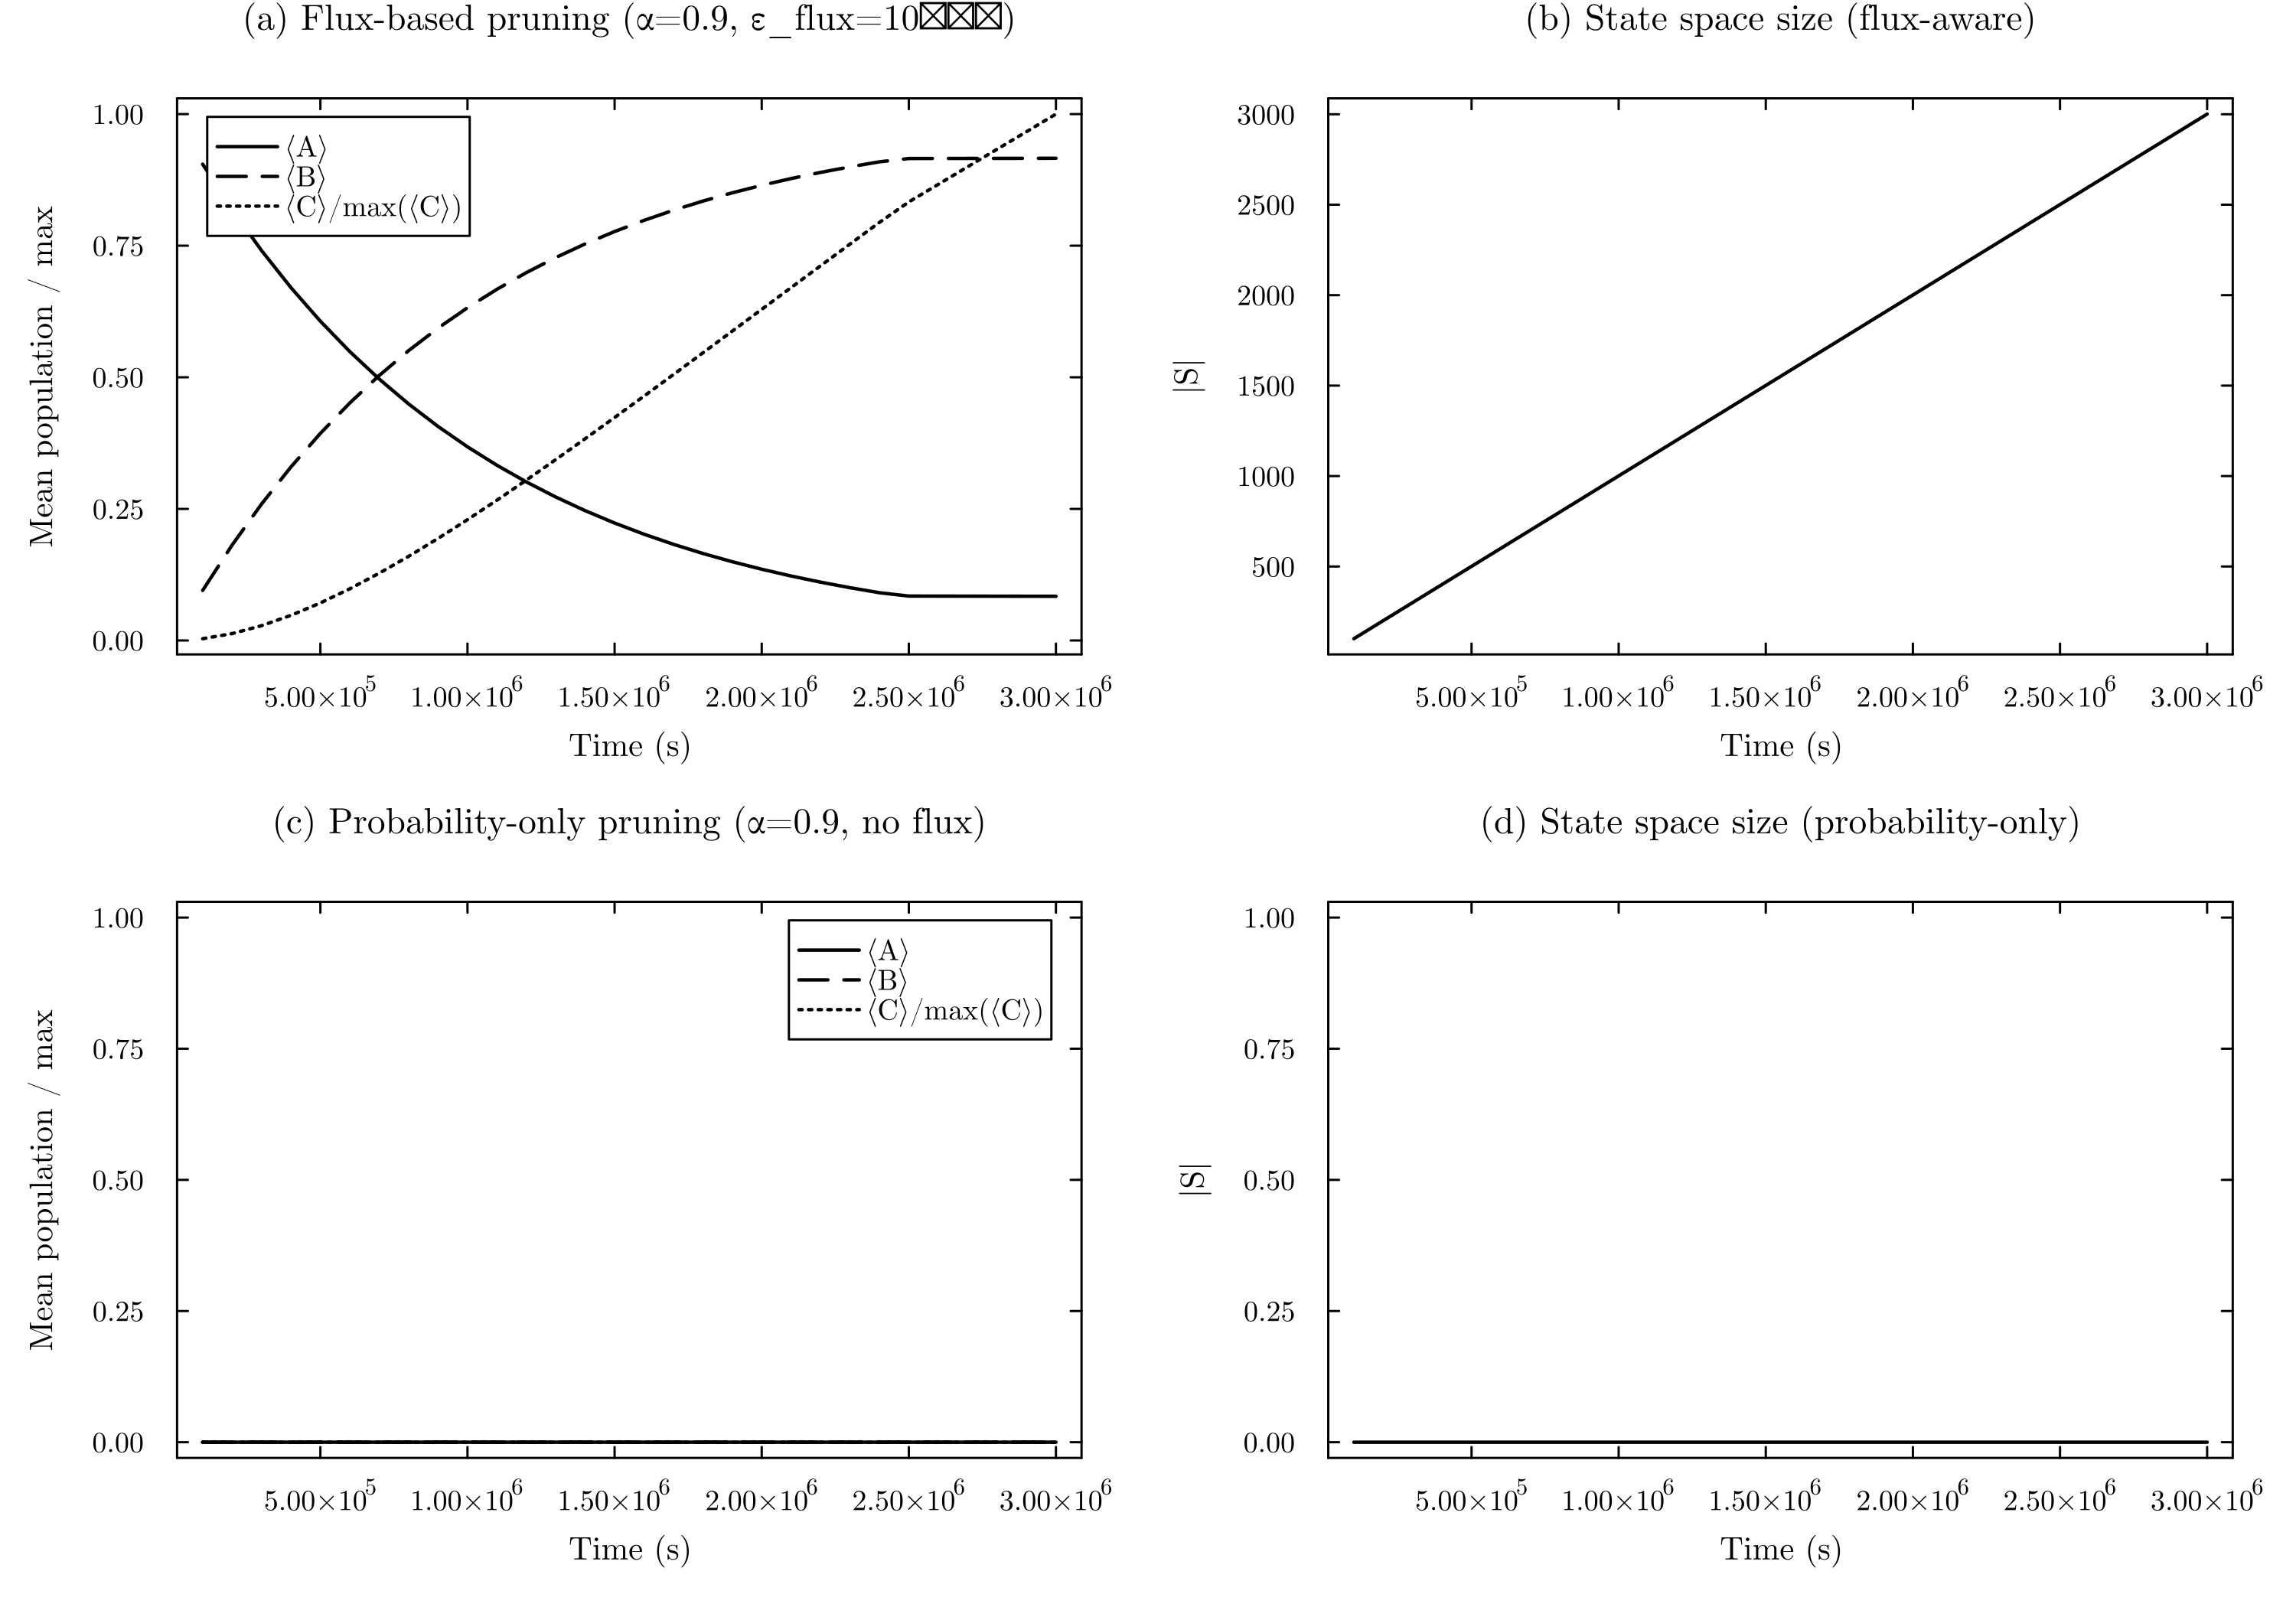
\includegraphics[width=\linewidth]{flux_vs_naive_comparison.png}
\caption{Comparison of flux-based and probability-only pruning on the bottleneck system. (a) Flux-based pruning ($\alpha=0.9$, $\epsilon_{\text{flux}}=10^{-12}$) correctly captures the transition dynamics with $\langle A \rangle$ decaying and $\langle C \rangle$ growing. (b) State space grows continuously to accommodate the advancing wave front while time step $\delta t$ adjusts adaptively. (c) Probability-only pruning ($\alpha=0.9$, no flux preservation) removes all intermediate states immediately, severing the connectivity pathway and causing all means to remain at initial values. (d) Only the initial state $(1,0,0)$ is retained throughout the simulation, creating a reducible generator.}
\label{fig:flux_vs_naive}
\end{figure}

The probability mass concentrates at the initial state $(1,0,0)$ and a traveling wave front at $(0,1,C_{\max}(t))$ where $C_{\max}$ grows approximately linearly with time. Intermediate states $(0,1,C)$ for $0 < C < C_{\max}$ form a critical connectivity pathway with negligible probability but significant flux. Tables~\ref{tab:bottleneck_diagnostics} and \ref{tab:prob_flux_rankings} quantify this structure at representative timepoints during the transition phase.

\begin{table}[htbp]
\centering
\caption{Distribution structure showing a quasi-bimodal behavior and bottleneck pathway characteristics during the stiff phase. The initial state $(1,0,0)$ gradually releases probability mass to the advancing tail $(0,1,C_{\max})$ of the distribution. Intermediate states along the pathway from $C=0$ to $C=C_{\max}$ maintain nearly constant flux despite having probability $p \lesssim 10^{-5}$. The pathway flux $\phi$ is computed as the total flux through intermediate bottleneck states and approximately equals $k_1 \cdot p(1,0,0)$.}
\label{tab:bottleneck_diagnostics}
\begin{tabular}{lccccc}
\hline
\textbf{Time (s)} & \textbf{$p(1,0,0)$} & \textbf{$C_{\max}$} & \textbf{$p(0,1,C_{\max})$} & \textbf{$|\mathcal{S}|$} & \textbf{Flux (s$^{-1}$)} \\
\hline
$1.0 \times 10^5$ & 0.905 & 1   & 0.095 & 4     & $9.0 \times 10^{-7}$ \\
$2.5 \times 10^5$ & 0.779 & 11  & 0.221 & 8     & $7.8 \times 10^{-7}$ \\
$5.1 \times 10^5$ & 0.600 & 33  & 0.400 & 36    & $6.0 \times 10^{-7}$ \\
$7.7 \times 10^5$ & 0.458 & 76  & 0.542 & 79    & $4.6 \times 10^{-7}$ \\
$3.0 \times 10^6$ & 0.081 & 8344 & 0.910 & 9124  & $8.4 \times 10^{-8}$ \\
\hline
\end{tabular}
\end{table}

\begin{table}[htbp]
\centering
\caption{Probability vs. flux rankings at early ($t=0$) and late ($t=3.0\times10^6$ s) times, demonstrating the disconnect between probability and flux. At $t=0$, the system has just initialized with all mass at $(1,0,0)$; zero-probability states $(0,1,0)$, $(0,1,1)$, $(0,1,2)$ carry the highest flux as they form the initial reaction pathway. At $t=3.0\times10^6$ s, state $(0,1,9121)$ near the wave front has negligible probability ($8\times10^{-4}$) but flux exceeding $10^{-4}$ s$^{-1}$. This is 100-fold higher than probability alone would suggest. Probability-only pruning would incorrectly remove all states except the top probability carrier, severing network connectivity.}
\label{tab:prob_flux_rankings}
\begin{tabular}{cccc}
\hline
\multicolumn{4}{c}{\textbf{Early time: $t = 1.0 \times 10^3$ s}} \\
\hline
\textbf{Rank} & \textbf{By probability} & \textbf{By flux} & \textbf{Flux (s$^{-1}$)} \\
\hline
1 & $(1,0,0)$, $p=0.999$ & $(0,1,2)$, $\phi=6.3\times10^{-5}$ & $6.3\times10^{-5}$ \\
2 & $(0,1,2)$, $p=6.3 \times 10^{-4}$ & $(0,1,1)$, $\phi=3.7\times10^{-5}$ & $3.7\times10^{-5}$ \\
3 & $(0,1,1)$, $p=3.7 \times 10^{-4}$ & $(0,1,0)$, $\phi=1.0\times10^{-6}$ & $1.0\times10^{-6}$ \\
4 & $(0,1,0)$, $p=1.0 \times 10^{-5}$ & $(1,0,0)$, $\phi=1.0\times10^{-6}$ & $1.0\times10^{-6}$ \\
\hline
\multicolumn{4}{c}{\textbf{Late time: $t = 3.0 \times 10^6$ s}} \\
\hline
\textbf{Rank} & \textbf{By probability} & \textbf{By flux} & \textbf{Flux (s$^{-1}$)} \\
\hline
1 & $(0,1,9122)$, $p=0.910$ & $(0,1,9121)$, $\phi=8.4\times10^{-5}$ & $8.4\times10^{-5}$ \\
2 & $(1,0,0)$, $p=0.081$ & $(0,1,2697)$, $\phi=2.0\times10^{-5}$ & $2.0\times10^{-5}$ \\
3 & $(0,1,9121)$, $p=8\times10^{-4}$ & $(0,1,4298)$, $\phi=3.1\times10^{-6}$ & $3.1\times10^{-6}$ \\
4 & $(0,1,9120)$, $p=2\times10^{-4}$ & $(0,1,4755)$, $\phi=3.2\times10^{-7}$ & $3.2\times10^{-7}$ \\
\hline
\end{tabular}
\end{table}

At early times ($t \sim 10^5$ s), the system exhibits a clear quasi-bimodal distribution with significant mass at both $(1,0,0)$ and the advancing front. As time progresses, probability mass transfers from the trapped state to the wave front, with $p(1,0,0)$ decreasing from 0.905 to 0.081 while $p(0,1,C_{\max})$ increases from 0.095 to 0.910 over the observed time range. The state space grows continuously from 4 to over 9000 states to accommodate the advancing front, with $C_{\max}$ increasing approximately linearly at rate $k_2 \approx 1$ s$^{-1}$ once $B=1$ is established.

Table~\ref{tab:prob_flux_rankings} reveals the critical disconnect between probability and flux rankings. At $t=1.0\times10^3$ s (shown with flux tolerance $\epsilon=10^{-3}$ to capture early dynamics), while $(1,0,0)$ dominates by probability with $p=0.999$, state $(0,1,2)$ at the wave front carries the highest flux of $6.3\times10^{-5}$ s$^{-1}$ despite having probability $p=6.3\times10^{-4}$—a flux-to-probability ratio of 100. State $(0,1,1)$ exhibits a similar pattern with flux $3.7\times10^{-5}$ s$^{-1}$ and probability $3.7\times10^{-4}$, while the bottleneck connector $(0,1,0)$ with $p=1.0\times10^{-5}$ carries flux comparable to the dominant state. At $t=3.0\times10^6$ s, this disconnect becomes even more pronounced: state $(0,1,9121)$ ranks third by probability with $p=8\times10^{-4}$ but first by flux with $\phi=8.4\times10^{-5}$ s$^{-1}$. Similarly, states $(0,1,2697)$ and $(0,1,4298)$ appear nowhere in the top probability rankings yet carry flux values of $2.0\times10^{-5}$ and $3.1\times10^{-6}$ s$^{-1}$, respectively. These states form the critical bottleneck chain connecting the trapped region at $(1,0,0)$ to the active wave front at $(0,1,9122)$.

The bottleneck pathway flux $\phi \approx k_1 \cdot p(1,0,0)$ decreases proportionally as mass depletes from the initial state, ranging from $9.0 \times 10^{-7}$ s$^{-1}$ at early times down to $8.4 \times 10^{-8}$ s$^{-1}$ at $t = 3 \times 10^6$ s. Despite this decreasing flux magnitude, the intermediate states maintain flux values that are orders of magnitude larger than their probabilities, as quantified in Table~\ref{tab:prob_flux_rankings}.

Figure~\ref{fig:flux_vs_naive} compares flux-based pruning against probability-only pruning. The flux-based method correctly preserves intermediate states despite their negligible probability, maintaining network connectivity and capturing the transition dynamics. State space growth is adaptive and continuous, expanding to accommodate the advancing wave front. The adaptive time step $\delta t$ begins at $\sim 10^5$ s and decreases to $\sim 10^3$ s during rapid transitions before stabilizing.

In contrast, probability-only pruning removes all states except $(1,0,0)$ immediately, creating a reducible generator where the initial state becomes absorbing. This severs the connectivity pathway entirely, causing all mean values to remain at their initial conditions: $\langle A \rangle = 1$, $\langle B \rangle = 0$, $\langle C \rangle = 0$ for all time. This method incorrectly predicts zero production of species $C$ when the correct answer shows $\langle C \rangle$ growing linearly with time to reach thousands by $t = 10^6$ s.

This example demonstrates that bottleneck states are essential for preserving network ergodicity and accurate long-time dynamics. Flux-based pruning correctly identifies and retains these states even when they carry negligible mass, while probability-based thresholds incorrectly remove them. The method successfully maintains connectivity across state spaces ranging from single-digit to thousands of states, adapting the representation as the distribution evolves.


\subsubsection{Experimental Error Analysis}
\begin{figure}[htbp]
\centering
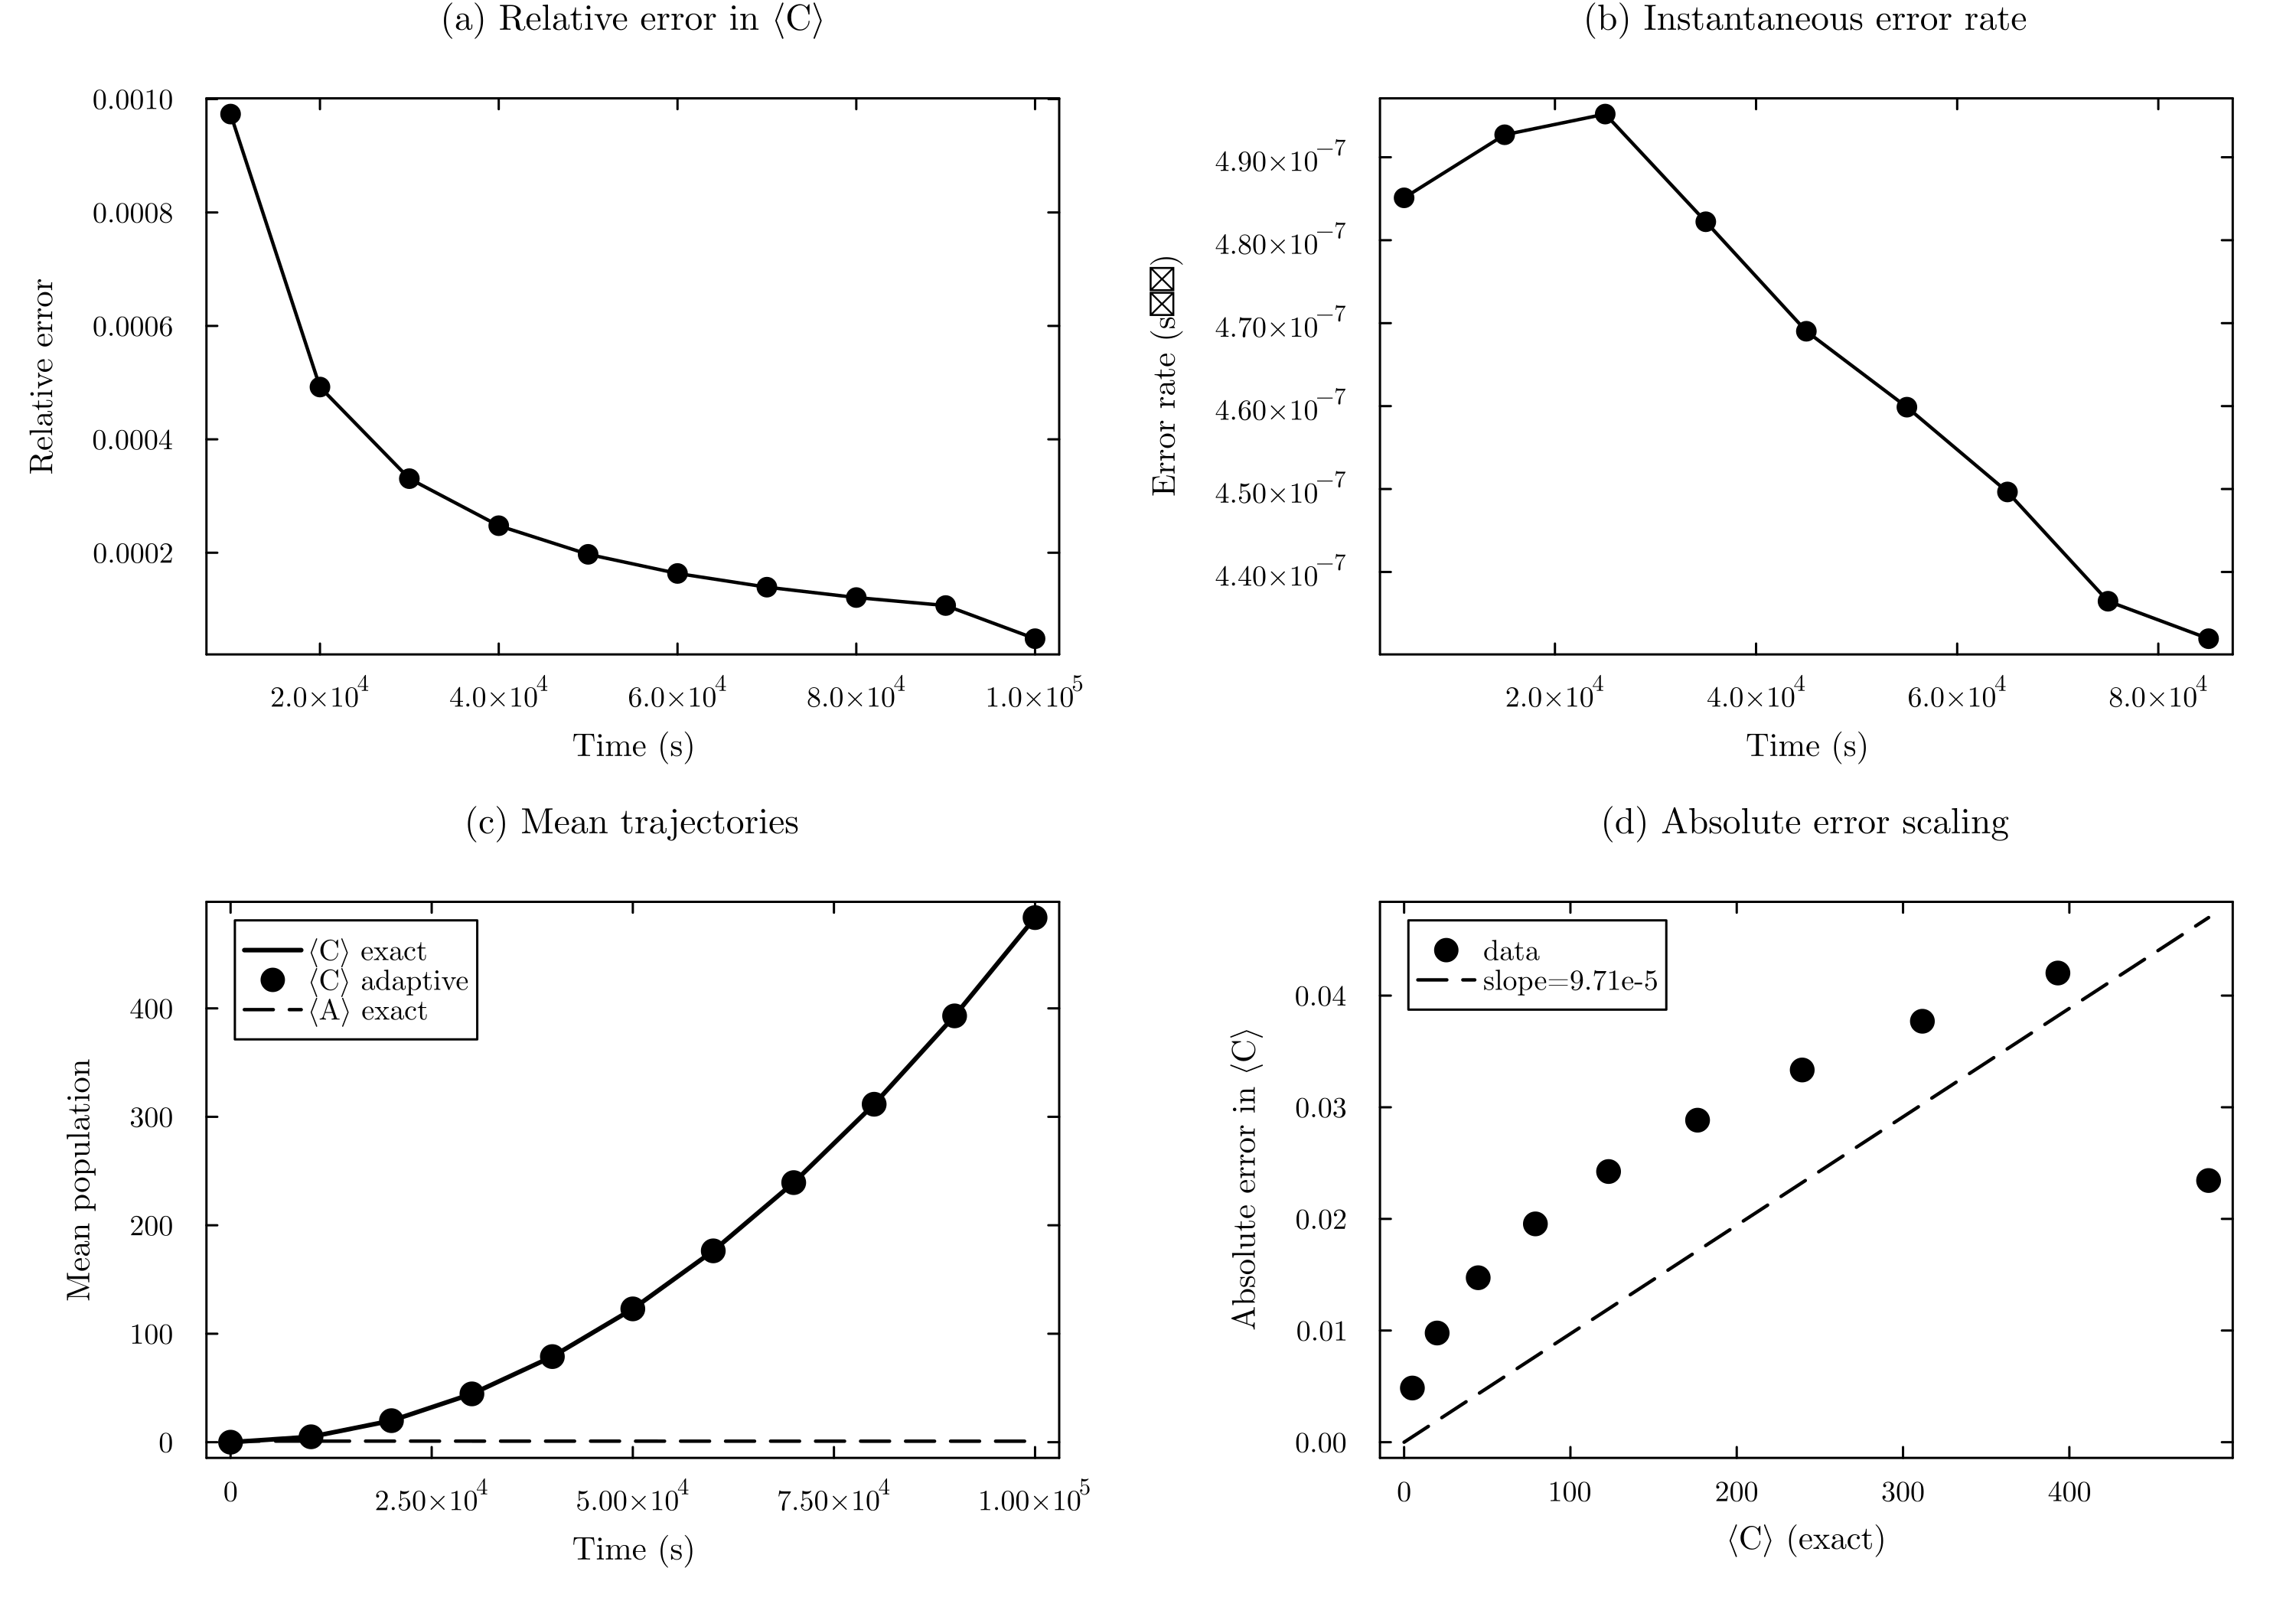
\includegraphics[width=\textwidth]{error_accumulation_analysis.png}
\caption{Error accumulation analysis over $10^5$ seconds with flux tolerance $\epsilon_{\text{flux}} = 10^{-6}$. (a) Relative error in mean of species $C$ decays from $0.1\%$ to $0.015\%$ as the distribution spreads. (b) Instantaneous error rate remains approximately constant at $4.9 \times 10^{-7}$ s$^{-1}$ throughout the stable region. (c) Mean trajectories for species $C$ (full FSP vs.\ adaptive) and species $A$ (reference). (d) Absolute error scales linearly with mean population: $\epsilon \approx 1.11 \times 10^{-4} \langle C \rangle$, corresponding to $0.01\%$ relative error.}
\label{fig:error_accumulation}
\end{figure}

The slowly expanding state-space of the bottleneck system allows us to experimentally compare the flux-aware adaptive FSP against the full FSP method over extended time periods. Because the bottleneck dynamics confine probability mass to a manageable region, we can compute the full FSP solution as a reference and directly measure the accuracy of our adaptive approach. We validate Corollary~\ref{cor:global-error} by comparing the adaptive FSP (quantile + flux-preserving pruning) against an exact FSP on a fixed state space $\{0,\ldots,2\} \times \{0,\ldots,2\} \times \{0,\ldots,10000\}$. The exact solution evaluates the matrix exponential at times $t \in \{0, 10^4, 2\times10^4, \ldots, 10^5\}$ s, while the adaptive method uses $\delta t = 10$ s steps with dynamic truncation.

Figure~\ref{fig:error_accumulation} shows error behavior over the full time interval. Panel (a) demonstrates that relative error in $\langle C \rangle$ decreases from $0.1\%$ to $0.015\%$ as the distribution spreads—the absolute error grows with the mean, but represents a shrinking fraction of the population. Panel (b) reveals constant instantaneous error rate of approximately $4.9 \times 10^{-7}$ s$^{-1}$, confirming the additive error accumulation predicted by Corollary~\ref{cor:global-error}. Panel (c) shows visually indistinguishable mean trajectories for species $C$. Panel (d) establishes linear error scaling $\epsilon \approx 1.11 \times 10^{-4} \langle C \rangle$, yielding $0.01\%$ relative error maintained across three orders of magnitude in population.

\begin{table}[htbp]
\centering
\caption{Distribution errors at $t = 10^5$ s.}
\label{tab:distribution_errors}
\begin{tabular}{lccc}
\hline
\textbf{Metric} & \textbf{Species $A$} & \textbf{Species $B$} & \textbf{Species $C$} \\
\hline
Mean (Adaptive) & $0.9903$ & $9.71 \times 10^{-3}$ & $474.6$ \\
Mean (Exact) & $0.9900$ & $9.95 \times 10^{-3}$ & $474.7$ \\
Absolute Error & $2.5 \times 10^{-4}$ & $2.5 \times 10^{-4}$ & $0.072$ \\
Relative Error & $0.025\%$ & $2.5\%$ & $0.015\%$ \\
\hline
\end{tabular}
\end{table}

Table~\ref{tab:distribution_errors} quantifies final-time accuracy. Species $C$ achieves $0.015\%$ relative error with absolute error $0.072$—the linear scaling $\epsilon \propto \langle C \rangle$ ensures errors remain proportional to population size. The adaptive state space contains $10{,}003$ states versus the exact method's $45{,}009$ states ($4.5\times$ reduction), though the adaptive space grows linearly in time as $C$ accumulates. Flux-based pruning correctly preserves low-probability bottleneck states at small $C$ values that remain connectivity-critical even as the distribution bulk moves to higher values. Aggressive probability pruning would sever these pathways and destroy long-time accuracy.

The results validate the error bound as $\mathcal{O}(10^{-4})$ relative error in means across $10^4$ time steps, constant error rate $\sim 5 \times 10^{-7}$ s$^{-1}$, and additive rather than multiplicative accumulation due to generator contraction.


\subsection{Stochastic Toggle Switch Model}

\begin{figure}[!htbp]
    \centering
    
\includegraphics[width=\linewidth]{toggle_switch_grid.pdf}
    \caption{
    Joint probability contours of the stochastic toggle switch at three representative time points (\(t\approx 2, 15, 30\)). 
    Columns correspond to time, while rows correspond to different adaptive--FSP configurations:
    (top) pruning mass \(0.3\) with no flux filter;
    (middle) pruning mass \(0.3\) with flux tolerance \(10^{-7}\);
    (bottom) pruning mass \(0.001\) with no flux filter.
    Black contour lines indicate probability levels, and dotted curves indicate the truncation boundary.
    The right column shows the corresponding state-space size trajectories.
    }
    \label{fig:toggle_results}
\end{figure}

The stochastic toggle switch models a genetic regulatory network where two proteins ($U$ and $V$) mutually repress each other via Hill-type kinetics~\cite{tian_stochastic_2006}. The forward reactions incorporate cooperativity with Hill coefficient $n=3$ to model mutual repression, while the reverse reactions represent degradation. Table~\ref{table:toggle} details the reaction network.


\begin{table}[!htbp]
\centering
\begin{tabular}{|c|c|c|}
\hline
\textit{Reaction} & \textit{Reaction Equation} & \textit{Parameter Values} \\
\hline
1 & \(\emptyset \xrightarrow{\eta\left(\alpha_1 + \frac{\beta_1K_1^3}{K_1^3+V^3}\right)} U\) & $\eta = 1.0$, $\alpha_1 = 20$, $\beta_1 = 400$, $K_1 = 100$ \\
2 & \(U \xrightarrow{d_1+\frac{s\gamma}{1+s}} \emptyset\) & $d_1 = 1.0$, $s = 0.1$, $\gamma = 1.0$ \\
3 & \(\emptyset \xrightarrow{\eta\left(\alpha_2 + \frac{\beta_2K_2^3}{K_2^3+U^3}\right)} V\) & $\eta = 1.0$, $\alpha_2 = 20$, $\beta_2 = 400$, $K_2 = 100$ \\
4 & \(V \xrightarrow{d_2} \emptyset\) & $d_2 = 1.0$ \\
\hline
\end{tabular}
\caption{Reactions and parameter values for the stochastic toggle switch model~\cite{tian_stochastic_2006, Dinh_2020}. Forward reactions incorporate Hill-type kinetics with cooperativity coefficient $n=3$ to capture mutual repression; reverse reactions represent degradation.}
\label{table:toggle}
\end{table}


The system exhibits bistability as probability mass accumulates in two spatially separated regions corresponding to high expression of one protein and low expression of the other. Noise-driven transitions between these stable states occur over long timescales, requiring the adaptive method to simultaneously maintain multiple disconnected regions of state space while tracking rare switching events.

We initialize at $(U, V) = (85, 5)$ with reaction rate parameters taken from~\cite{Dinh_2020} and volume scaling factor $\eta = 100$. The simulation evolves over $t \in [0, 30]$ with initial time step $\delta t = 0.05$. This setup produces a bimodal distribution by the final time, with stable peaks near $(U, V) \approx (90, 10)$ and $(10, 90)$.

Figure~\ref{fig:toggle_results} examines the evolution of the joint distribution under three variants of the adaptive FSP scheme.  
In all cases, the system is initialized at \((U,V)=(85,5)\) and simulated to \(t=30\).  
Each column of the figure shows contour lines of \(\log_{10}(p)\) at three representative times, and each row corresponds to one truncation scheme.

With pruning mass \(0.3\) and no flux filter (top row), the state space expands rapidly after initialization, resolving the dominant drift into the lower metastable well.  
However, the truncation boundary is somewhat irregular and tends to either lag behind or overshoot the motion of the probability mass.  
This behavior reflects the fact that pruning is governed solely by a coarse quantile threshold as many intermediate transition states fall below the quantile cutoff and may be removed prematurely, while other regions are retained longer than necessary.

Introducing a flux tolerance of \(10^{-7}\) while keeping the pruning mass at \(0.3\) produces a dramatically more stable truncation (middle row).  
Here the boundary follows the outermost probability contours much more tightly, especially during the intermediate regime (\(t\approx 10{-}20\)) when the distribution stretches along the switching manifold connecting the two wells.  
The flux constraint protects states that carry even a small outward probability flow, preventing the removal of structurally important low-probability connectors.  
The resulting state space is noticeably smaller than in the quantile-only case, while still preserving the correct geometric structure of the distribution.

Reducing the pruning mass to \(0.001\) without a flux filter (bottom row) results in the most conservative truncation.  
The boundary expands to include a wide region of low-probability states, producing the largest active state space among the three experiments.  
Although this approach avoids under-truncation entirely, it incurs a substantial computational cost and offers little improvement over the flux-filtered configuration. Across all three settings, the adaptive FSP framework correctly resolves the emergence and separation of the two metastable wells. The comparison demonstrates the role of the flux tolerance as it preserves accuracy in the thin transition region without requiring an excessively small pruning mass, leading to a substantially more efficient state-space representation.  


\subsection{Oscillatory Dynamics in the Oregonator Model}

We examine the Oregonator model, a reduced representation of the Belousov-Zhabotinsky oscillating chemical reaction developed by Field and Noyes \cite{field_noyes}. This three-species system captures the essential autocatalytic and inhibitory feedback mechanisms that generate sustained chemical oscillations. The Oregonator serves as a stringent test for numerical methods due to its combination of multiple timescales, relaxation oscillations, and sensitivity to parameter variations. The model consists of five elementary reactions involving three intermediate species: $X$ (HBrO$_2$), $Y$ (Br$^-$), and $Z$ (Ce$^{4+}$). The complete reaction network is presented in Table \ref{table:oregonator}. 

The reaction network exhibits three distinct dynamical phases. The autocatalytic reaction (R3) drives explosive growth of $X$ when inhibitor $Y$ is depleted. The quadratic termination (R4) prevents unbounded growth at high $X$ concentrations. The recovery reaction (R5) slowly regenerates $Y$ from $Z$, resetting the cycle. Following Gillespie's methodology \cite{Gillespie1977}, we determine rate constants by analyzing the deterministic steady state. At equilibrium, the net flux for each species vanishes:
\begin{align}
\frac{dN_X}{dt} &= k_1 N_Y - k_2 N_X N_Y + k_3 N_X - 2k_4 N_X^2 = 0, \\
\frac{dN_Y}{dt} &= -k_1 N_Y - k_2 N_X N_Y + k_5 N_Z = 0, \\
\frac{dN_Z}{dt} &= k_3 N_X - k_5 N_Z = 0.
\end{align}
We specify the steady-state populations as $(N_X^*, N_Y^*, N_Z^*) = (500, 1000, 2000)$ molecules, placing the system in the oscillatory regime. From the third equation, $k_3 N_X^* = k_5 N_Z^*$, which implies $\mu_3 = \mu_5$, where $\mu_i = k_i N_i^*$ denotes the steady-state flux through reaction $i$. Defining the characteristic fluxes $\mu_1^* = k_1 N_Y^* = 2000$ s$^{-1}$ and $\mu_2^* = k_2 N_X^* N_Y^* = 50000$ s$^{-1}$, we obtain the rate constants summarized in Table~\ref{table:oregonator}.

\begin{table}[!htbp]
\centering
\caption{Oregonator reaction network with mass-action kinetics and rate constants determined by steady-state flux balance at $(N_X^*, N_Y^*, N_Z^*) = (500, 1000, 2000)$ molecules.}
\label{table:oregonator}
\begin{tabular}{|c|l|c|l|}
\hline
\textit{Rxn} & \textit{Reaction} & \textit{Rate Constant} & \textit{Propensity Function}\\
\hline
1 & $Y \xrightarrow{k_1} X$ & $k_1 = 2.0$ s$^{-1}$ & $k_1 N_Y$ \\
2 & $X + Y \xrightarrow{k_2} \varnothing$ & $k_2 = 0.1$ molec$^{-1}$s$^{-1}$ & $k_2 N_X N_Y$ \\
3 & $X \xrightarrow{k_3} 2X + Z$ & $k_3 = 104$ s$^{-1}$ & $k_3 N_X$ \\
4 & $2X \xrightarrow{k_4} \varnothing$ & $k_4 = 0.016$ molec$^{-1}$s$^{-1}$ & $k_4 \frac{N_X(N_X-1)}{2}$ \\
5 & $Z \xrightarrow{k_5} Y$ & $k_5 = 26$ s$^{-1}$ & $k_5 N_Z$ \\
\hline
\end{tabular}
\end{table}

These parameters yield a period of approximately 0.85 time units with timescale separation spanning three orders of magnitude, specifically, the autocatalytic amplification (R3) at $k_3 = 104$ s$^{-1}$ drives explosive bursts, recovery (R5) operates at intermediate rate $k_5 = 26$ s$^{-1}$, and initiation (R1) proceeds slowly at $k_1 = 2.0$ s$^{-1}$. At steady-state concentrations, the inhibitory consumption (R2) dominates with flux $\mu_2^* = 50000$ s$^{-1}$.

At the steady-state initial condition, the total flux is $\Phi_{\mathrm{total}} \approx 158{,}000\,\text{s}^{-1}$ and the maximum individual propensity is $\lambda_{\max} = k_3 N_X^* = 52{,}000\,\text{s}^{-1}$, giving spatial stiffness ratio $\kappa \approx 0.33$.
By Corollary~\ref{cor:expansion-depth} with $\varepsilon_{\Delta t} = 1$, the required expansion depth is $d_{\min} = \lceil \kappa\,\varepsilon_{\Delta t} \rceil = 1$, so we set \texttt{expansion\_depth = 1}.

Figure \ref{fig:oregonator_fsp_results} presents results over four complete oscillation cycles. The adaptive time step (panel a) varies over two orders of magnitude from $\Delta t_{\min} \approx 0.005$ during autocatalytic bursts to $\Delta t_{\max} \approx 0.04$ during recovery, tracking the instantaneous system flux and local stiffness.

The state space size (panel b) demonstrates excellent compression efficiency. Based on the observed mean trajectory ranges in panel c, a rectangular bounding box would require approximately $4000 \times 7000 \times 11000 \approx 3 \times 10^{11}$ states. Yet the adaptive method maintains only 50-2000 active states throughout the simulation: $|S| \approx 50$ during the recovery phase when the distribution concentrates tightly, expanding to $|S| \approx 2000$ during autocatalytic bursts when Poisson fluctuations spread the distribution. This achieves compression ratio $\approx 10^8:1$ while maintaining rigorous flux-based error control.

The mean trajectories (panel c) exhibit characteristic relaxation oscillations. Species $X$ spikes from near-zero to 6000 molecules in $< 0.1$ time units, consistent with the fast autocatalytic timescale $1/k_3$. Species $Y$ depletes rapidly during bursts via reactions R1 and R2, then recovers slowly via R5. Species $Z$ accumulates to 10000 molecules during each burst and decays with characteristic time $1/k_5 \approx 0.04$ time units. The phase relationships reflect the feedback structure where $Y$ depletion enables $X$ growth, $X$ growth produces $Z$, and $Z$ accumulation regenerates $Y$.

The phase space projections (panels d-f) reveal the limit cycle attractor. The $X$-$Y$ plane (panel d) shows the relaxation oscillation "knee": slow recovery where $Y$ increases with $X$ near zero, followed by rapid burst when $X$ spikes and $Y$ depletes. The $X$-$Z$ plane (panel e) displays an elliptical cycle with $Z$ lagging $X$ due to production-decay dynamics. The $Y$-$Z$ plane (panel f) demonstrates phase lag between inhibitor depletion and product accumulation. Counter-clockwise circulation in all projections confirms stable periodicity despite stochastic dynamics.
\begin{figure}[!htbp]
    \centering
    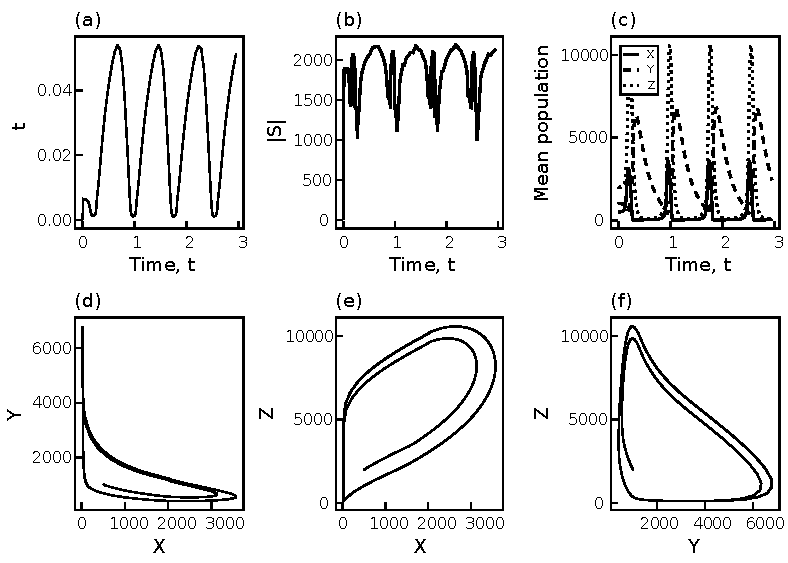
\includegraphics[width=\linewidth]{orag.pdf}
    \caption{Adaptive FSP simulation of the Oregonator system. (a) Adaptive time step variation tracking instantaneous system stiffness. (b) Dynamic state space size showing compression ratio of $\sim 10^8:1$ relative to the theoretical state space of $3.6 \times 10^{11}$ states. (c) Mean population trajectories for species $X$ (solid), $Y$ (dash-dot), and $Z$ (dotted). (d-f) Phase space projections revealing the limit cycle attractor with intrinsic stochastic fluctuations.}
    \label{fig:oregonator_fsp_results}
\end{figure}

\subsection{Stiff Dynamics in the Robertson Autocatalytic System}

The Robertson system provides a severe test of numerical methods through its extreme stiffness, with reaction rates spanning nine orders of magnitude. Originally formulated by Robertson \cite{Robertson1967} for testing ODE solvers, this autocatalytic network has become a standard benchmark for stochastic simulation algorithms. The system involves three species undergoing the reactions shown in Table \ref{table:robertson}, with rate constants $k_1 = 0.04$ s$^{-1}$, $k_2 = 3 \times 10^7$ molecule$^{-1}$s$^{-1}$, and $k_3 = 10^4$ molecule$^{-1}$s$^{-1}$. This yields a stiffness ratio of $k_2/k_1 \approx 7.5 \times 10^8$, creating a temporal scale separation where the fast autocatalytic reaction R2 operates nearly a billion times faster than the slow initiation reaction R1.

\begin{table}[!htbp]
\centering
\caption{Robertson autocatalytic reaction system with extreme rate constant disparity}
\label{table:robertson}
\begin{tabular}{|c|l|c|l|}
\hline
\textit{Rxn} & \textit{Reaction} & \textit{Rate Constant} & \textit{Propensity Function} \\
\hline
1 & $A \xrightarrow{k_1} B$ & $k_1 = 0.04$ s$^{-1}$ & $a_1 = k_1 N_A$ \\
2 & $2B \xrightarrow{k_2} B + C$ & $k_2 = 3 \times 10^7$ molec$^{-1}$s$^{-1}$ & $a_2 = k_2 \frac{N_B(N_B-1)}{2}$ \\
3 & $B + C \xrightarrow{k_3} A + C$ & $k_3 = 10^4$ molec$^{-1}$s$^{-1}$ & $a_3 = k_3 N_B N_C$ \\
\hline
\end{tabular}
\end{table}

\begin{figure}[!htbp]
    \centering
    
\includegraphics[width=\linewidth]{simulation_results.pdf}
    \caption{Adaptive FSP simulation of the Robertson system over eight decades of time ($10^{-5}$ to $10^5$ s). (a) Mean population trajectories for species $A$ (solid), $B$ (dashed), and $C$ (dotted) showing three-phase dynamics: slow initiation, explosive autocatalysis, and protracted equilibration. (b) Dynamic state space size achieving $\sim 10^4:1$ compression relative to the theoretical space of $3 \times 10^7$ states. (c) Adaptive time step spanning seven orders of magnitude in response to changing flux. (d) Total flux tracking system activity and guiding both time step and state space adaptation.}
    \label{fig:robertson_results}
\end{figure}

The system conserves total mass: $N_{\text{tot}} = N_A + N_B + N_C = 10000$ molecules. We initialize with $(N_A, N_B, N_C) = (10000, 0, 0)$, triggering characteristic three-phase dynamics that span eight decades of time. Figure~\ref{fig:robertson_results} demonstrates how the adaptive FSP method navigates this extreme stiffness through coordinated adjustment of time step, state space size, and flux monitoring.

At initialization, only R1 is active, giving $\Phi_{\mathrm{total}} = \lambda_{\max} = k_1 N_A = 400\,\text{s}^{-1}$ and hence $\kappa = 1$.
As $B$ accumulates, R2 rapidly comes to dominate both $\lambda_{\max}$ and $\Phi_{\mathrm{total}}$, keeping $\kappa \approx 1$ throughout the simulation.
By Corollary~\ref{cor:expansion-depth} with $\varepsilon_{\Delta t} = 0.01$, this gives $d_{\min} = \lceil \kappa\,\varepsilon_{\Delta t} \rceil = 1$, so we set \texttt{expansion\_depth = 1}.

During the initial phase ($t < 10^{-2}$ s), species $A$ converts slowly to $B$ through reaction R1 at rate 0.04 s$^{-1}$. Panel (a) shows $A$ decreasing from 10000 molecules while $B$ (scaled $\times 10^4$) accumulates slowly and $C$ remains near zero. Time steps (panel c) remain near $\Delta t \approx 10^{-4}$ s, matching the dominant flux timescale. The state space (panel b) contains fewer than 50 states, reflecting the narrow distribution around the nearly deterministic trajectory. The flux threshold (panel d) hovers around 400 s$^{-1}$, dominated by reaction R1 with propensity $k_1 N_A \approx 400$ s$^{-1}$. This continues until $B$ reaches approximately 0.3 molecules near $t \approx 10^{-2}$ s.

The system then enters explosive transient phase ($10^{-2}$ s $< t < 10^2$ s) driven by reaction R2. Time steps contract to resolve the explosive dynamics, while the state space expands to over 2000 states as autocatalytic bursts amplify stochastic fluctuations scaling as $\sqrt{N_B}/N_B$. The flux threshold peaks near 800 s$^{-1}$. Using conservation law $N_A + N_B + N_C = 10000$ with observed ranges $N_A \in [0, 10000]$ and $N_B \in [0, 10]$, a rectangular bounding box requires approximately $10^5$ states. The adaptive method maintains only 2000 states at peak, achieving compression ratio $50:1$.

Following the transient ($t > 10^2$ s), reaction R3 slowly regenerates $A$ from $B$ and $C$, driving toward quasi-equilibrium near $(N_A, N_B, N_C) \approx (10000, 0, 0)$. Time steps increase progressively to $\Delta t \approx 10^2$ s by $t = 10^5$ s, spanning six orders of magnitude and the state space contracts to 500-1000 states as the distribution concentrates near quasi-equilibrium. The flux threshold decreases to approximately 100 s$^{-1}$ by $t = 10^4$ s, confirming approach to steady state.


\subsection{Performance Evaluation of Matrix Construction}

In this subsection we evaluate the matrix construction strategy introduced in Section~\ref{sec:matrix_construction}. The forward enumeration approach constructs the generator by iterating through reactions for each state, directly computing destination states as $y = x + \nu_k$. We benchmark this strategy against a standard implementation that uses backward state expansion on the Oregonator, ROBER, and toggle switch models.

Figure~\ref{fig:benchmark} and Table~\ref{tab:benchmark} quantify the performance difference on the ROBER model using $10^4$ trials via BenchmarkTools.jl~\cite{BenchmarkTools.jl-2016}. The benchmark captures a representative time step at $t \approx 170$ where the state space expands from 1106 to 1431 states. Standard construction exhibits median execution time of 6.95~ms with moderate variability (std. dev. 2.33~ms), while forward enumeration achieves 0.54~ms median time (std. dev. 1.12~ms), a 12.9$\times$ speedup. The cumulative distribution functions reveal that forward enumeration completes $>99\%$ of trials by 3~ms, whereas standard construction requires $>10$~ms for comparable completion rates.

\begin{figure}[!htbp]
\centering

\includegraphics[width=\textwidth]{benchmark_comparison.pdf}
\caption{Performance comparison of standard construction (solid line) and forward enumeration (dashed line) at $t \approx 170$ with state space sizes 1106 $\to$ 1431. (a) Probability density functions on logarithmic scale with median markers at 6.95~ms and 0.54~ms. (b) Cumulative distribution functions showing 12.9$\times$ speedup: forward enumeration completes 50\% of trials by 0.54~ms versus 6.95~ms for standard construction.}
\label{fig:benchmark}
\end{figure}

\begin{table}[h]
\centering
\caption{Benchmark statistics for matrix construction methods on ROBER model at $t \approx 170$ (state space sizes 1106 $\to$ 1431).}
\label{tab:benchmark}
\begin{tabular}{lccc}
\hline
Method & Median (ms) & Mean (ms) & Std. Dev. (ms) \\
\hline
Standard construction & 6.95 & 7.38 & 2.33 \\
Forward enumeration & 0.54 & 0.71 & 1.12 \\
\hline
Speedup & 12.9$\times$ & 10.4$\times$ & --- \\
\hline
\end{tabular}
\end{table}
Figure~\ref{fig:speed_comparison} demonstrates cumulative impact across three benchmark systems. The Oregonator (panel a) exhibits oscillatory state space dynamics with cost spikes exceeding $10^{-2}$~s during rapid expansion phases under standard construction; forward enumeration maintains cost below $10^{-3}$~s throughout. The stiff ROBER system (panel b) shows pronounced cost fluctuations between $10^{-3}$~s and $10^{-1}$~s with standard construction, reduced to approximately $10^{-4}$~s with forward enumeration. The toggle switch (panel c) demonstrates the largest proportional gain, with forward enumeration reducing per-step cost from $\sim$$10^{0}$~s to below $10^{-1}$~s.

\begin{figure}[!htbp]
\centering

\includegraphics[width=\textwidth]{speed.pdf}
\caption{Wall-clock time per integration step for FSP simulations with forward enumeration (solid) and standard construction (dotted). (a) Oregonator. (b) ROBER. (c) Toggle switch. Forward enumeration consistently outperforms standard construction across all systems.}
\label{fig:speed_comparison}
\end{figure}

Table~\ref{tab:walltime} summarizes total simulation times. The toggle switch achieves the largest speedup at 9.8$\times$ (364~s reduced to 37~s), benefiting from slower reaction timescales and compact state space geometry. The Oregonator and ROBER systems achieve 3.9$\times$ and 3.5$\times$ speedups respectively (4000~s $\to$ 1093~s and 10421~s $\to$ 3015~s). The consistent performance gains across diverse system types demonstrate that forward enumeration is the preferred construction method.

\begin{table}[h]
\centering
\caption{Total wall-clock times for complete FSP simulations.}
\label{tab:walltime}
\begin{tabular}{lccc}
\hline
System & Standard (s) & Optimized (s) & Speedup \\
\hline
Oregonator & 4000 & 1093 & 3.9$\times$ \\
ROBER & 10421 & 3015 & 3.5$\times$ \\
Toggle switch & 364 & 37 & 9.8$\times$ \\
\hline
\end{tabular}
\end{table}

\subsection{Comparison with Krylov-FSP-SSA}
\label{sec:comparison}

To contextualize the flux-based adaptive FSP against existing methods, we compare with the Krylov-FSP-SSA algorithm of Vo and Sidje~\cite{Sidje2015}, reviewed in detail by Dinh and Sidje~\cite{Dinh2016}. This baseline shares the same expand--evolve--prune skeleton and Krylov matrix exponential integrator but differs in three key respects: (i) pruning uses a hard probability threshold with no flux protection, (ii) time stepping uses a mass-conservation accept/reject criterion (halving $\tau$ when the retained probability mass falls below $1 - \varepsilon$) rather than the flux-adaptive rule $\Delta t = \varepsilon_{\Delta t}/\Phi_{\mathrm{total}}$, and (iii) expansion is SSA-driven with $r$-step reachability enumeration. These differences isolate the effect of flux-aware pruning and flux-adaptive time stepping on the three benchmark systems.

\paragraph{Oregonator.}
Table~\ref{tab:comparison_oregonator} and Figure~\ref{fig:oregonator_comparison} compare the two methods on the Oregonator system over $[0, 0.11]$.
The flux-based adaptive FSP completes the simulation in 33\,s using 26 snapshots with a maximum active set of 1{,}003 states, while the Krylov-FSP-SSA method, using a fixed step $\tau = 10^{-6}$ (the largest step that avoids numerical overflow in the Krylov exponential), reaches only $t = 0.003$ (2.7\% of the time horizon) after 3{,}000 iterations and 74\,s of wall time, with an active set that grows to 13{,}294 states. The state space explosion (panel~(a)) arises because the probability-only pruning threshold ($\varepsilon = 10^{-2}$) retains many states with small probability that the flux-based rule would prune, while failing to identify the dynamically essential boundary states. The time step comparison (panel~(b)) illustrates the core advantage of flux-adaptive stepping: the adaptive FSP adjusts $\Delta t$ from $1.4\times10^{-6}$ to $1.9\times10^{-5}$ in response to the instantaneous total flux, whereas the Krylov-FSP-SSA method is locked at $\tau = 10^{-6}$ because larger steps cause mass loss exceeding the tolerance.

\begin{table}[!htbp]
\centering
\caption{Oregonator comparison: flux-based adaptive FSP vs.\ Krylov-FSP-SSA.}
\label{tab:comparison_oregonator}
\begin{tabular}{lcc}
\hline
Metric & Adaptive FSP & Krylov-FSP-SSA \\
\hline
Wall time (s) & 33 & 74 \\
Snapshots / Iterations & 26 & 3{,}000 \\
Time reached & 0.11 (complete) & 0.003 (2.7\%) \\
Max $|S|$ & 1{,}003 & 13{,}294 \\
Final $|S|$ & 1{,}003 & 13{,}272 \\
Rejections & --- & 0 \\
\hline
\end{tabular}
\end{table}

\begin{figure}[!htbp]
    \centering
    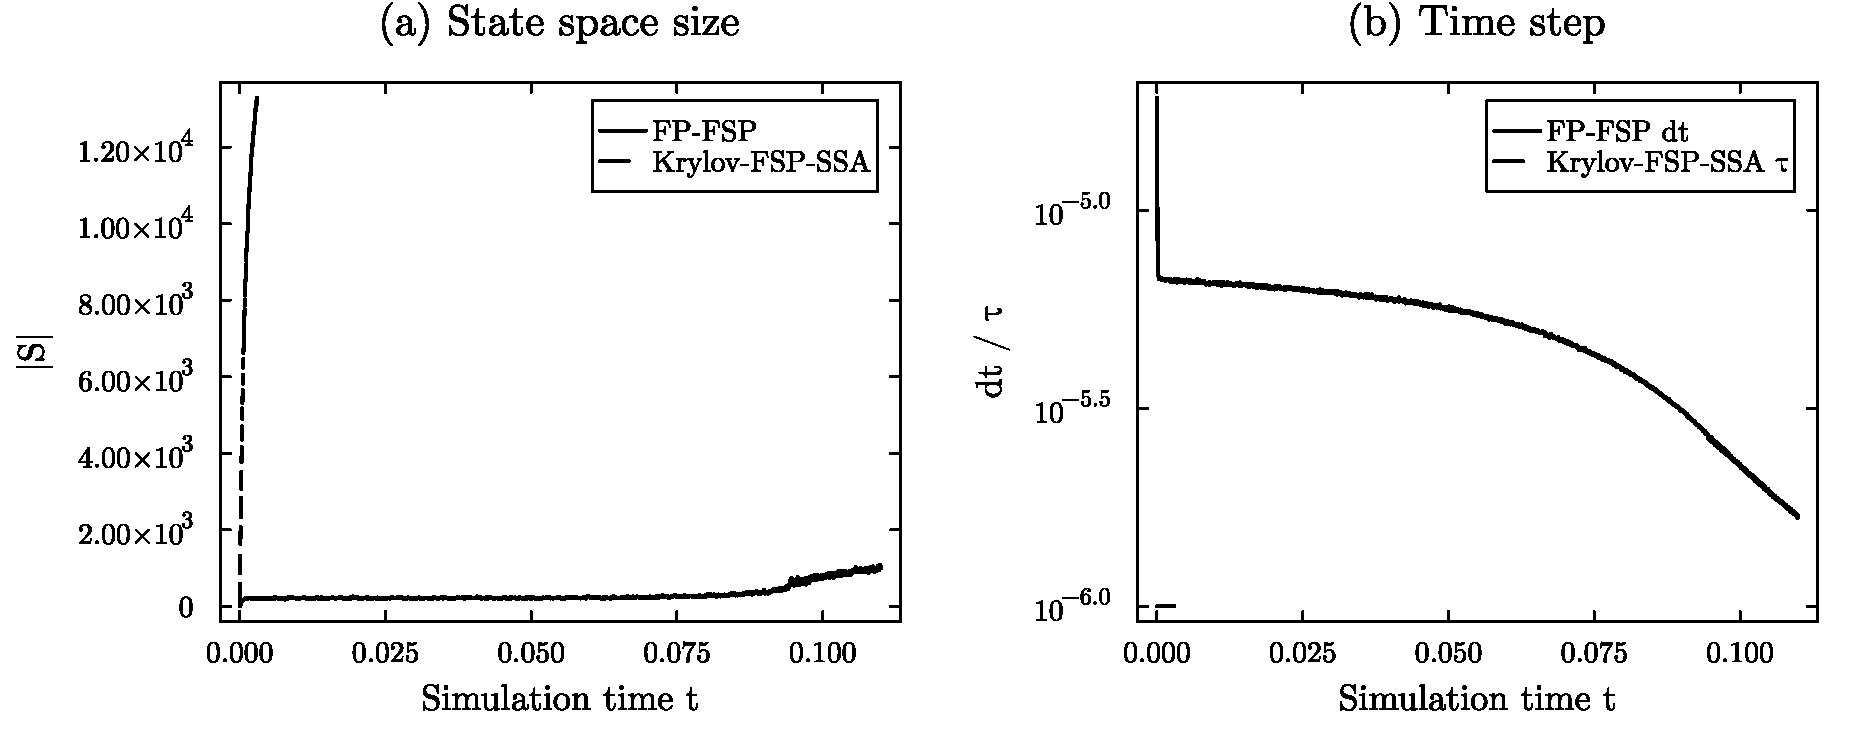
\includegraphics[width=\linewidth]{oregonator_comparison.pdf}
    \caption{Oregonator: FP-FSP (solid) vs.\ Krylov-FSP-SSA (dashed). (a) State space size: Krylov-FSP-SSA grows to ${\sim}13{,}300$ states without flux-based pruning, while FP-FSP maintains $<$1{,}100. (b) Time step: FP-FSP adjusts $\Delta t$ from $1.4\times10^{-6}$ to $1.9\times10^{-5}$; Krylov-FSP-SSA is fixed at $\tau = 10^{-6}$.}
    \label{fig:oregonator_comparison}
\end{figure}

\paragraph{Bottleneck.}
Table~\ref{tab:comparison_bottleneck} and Figure~\ref{fig:bottleneck_comparison} compare the methods on the bottleneck system ($A \to B \to B + C$, $k_1 = 10^{-6}$, $k_2 = 0.1$) over $[0, 10^4]$. The flux-based adaptive FSP uses a fixed time step $\delta t = 1/k_2 = 10$\,s (because the flux-adaptive formula $\varepsilon_{\Delta t}/\Phi_{\mathrm{total}} \approx 10^6$\,s at $t{=}0$ would take one giant step from $t{=}0$ to $t_f$, missing all $C$-states), completes in 1.0\,s with 1{,}000 steps, and achieves $\langle C \rangle = 4.978$ (${<}0.1\%$ error). The faithfully-implemented Krylov-FSP-SSA (Algorithm~2 of~\cite{VoSidje2016}; $\varepsilon = 10^{-2}$, $\tau_{\mathrm{init}} = 100$, $r = 1$, $\mathtt{droptol} = 10^{-10}$) also reaches $t_f$ in just 7 accepted steps, but produces $\langle C \rangle = 0.12$ (40$\times$ underestimate).

The failure mechanism is \emph{wavefront truncation}, not connectivity loss. With $\mathtt{droptol} = 10^{-10}$, the connector state $(0,1,0)$ carries $p(B{=}1) \approx k_1 t \sim 10^{-4}$--$10^{-2} \gg 10^{-10}$ and is correctly retained throughout ($\langle B \rangle = 0.010$ at $t_f$, consistent with $k_1 t_f = 10^{-2}$). The failure arises instead because no probability is lost to the projection boundary ($\sum w \approx 1$ at every step), so $\tau$ doubles after each accepted step, growing from 100 to 3{,}700\,s. Meanwhile, the depth-$r{=}1$ expansion adds only one new $C$-state per step. After 7 steps the projection contains just 14 states (covering only $C \leq 12$), while the true conditional distribution $C\mid B{=}1$ has spread over $[0,\, k_2 t_f] \approx [0, 1{,}000]$. The matrix exponential correctly propagates probability within the truncated projection, but flux to $C \geq 13$ is silently discarded because those rows are absent from the generator; the mass-conservation criterion $\sum w \geq 1 - \varepsilon(t{+}\tau)/t_f$ does not detect this because missing-row truncation does not reduce $\sum w$ within the projection. The flux-based method avoids this failure by using a fixed step $\delta t = 1/k_2 = 10$\,s, ensuring that the depth-1 expansion keeps pace with the physical probability wavefront.

\begin{table}[!htbp]
\centering
\caption{Bottleneck comparison ($t_f = 10^4$): FP-FSP (flux-adaptive $\delta t$) vs.\ Krylov-FSP-SSA (Algorithm~2 of~\cite{VoSidje2016}, $\varepsilon=10^{-2}$, $\tau_{\mathrm{init}}=100$, $r=1$). Both methods retain the connector state $B{=}1$, but Krylov-FSP-SSA underestimates $\langle C \rangle$ by 40$\times$ due to wavefront truncation.}
\label{tab:comparison_bottleneck}
\begin{tabular}{lcc}
\hline
Metric & FP-FSP & Krylov-FSP-SSA \\
\hline
Wall time (s) & 1.0 & ${<}0.1$ \\
Steps / Iterations & 1{,}000 ($\delta t=10$, adaptive) & 7 ($\tau$: $100 \to 3{,}700$) \\
Time reached & $10^4$ (complete) & $10^4$ (complete) \\
Final $\langle C \rangle$ & 4.978 & 0.12 (40$\times$ low) \\
Final $\langle B \rangle$ & 0.010 & 0.010 (both correct) \\
Final $|\mathcal{S}|$ & 1{,}001 & 14 \\
$B{=}1$ retained & Yes & Yes \\
\hline
\end{tabular}
\end{table}

\begin{figure}[!htbp]
    \centering
    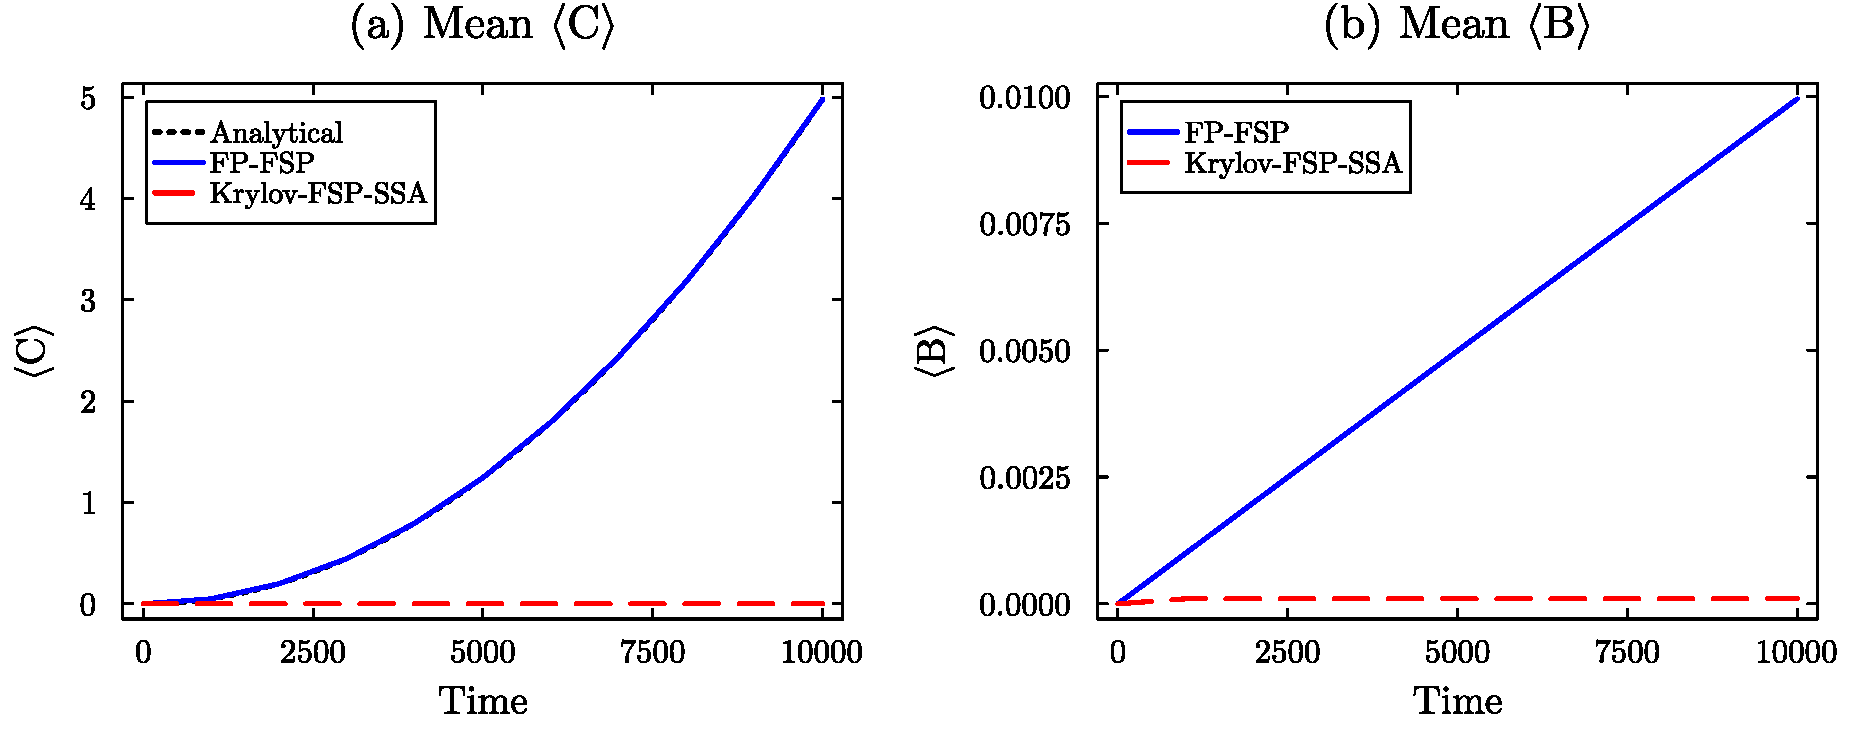
\includegraphics[width=\linewidth]{bottleneck_comparison.pdf}
    \caption{Bottleneck system ($A \to B \to B+C$, $k_1=10^{-6}$, $k_2=0.1$, $t_f=10^4$). FP-FSP (solid) vs.\ Krylov-FSP-SSA (dashed); dotted line with star markers: analytical solution. (a) Mean $\langle C \rangle$: FP-FSP tracks the analytical reference with ${<}0.1\%$ error; Krylov-FSP-SSA covers $[0,t_f]$ in only 7 giant steps ($\tau$ grows from 100 to 3{,}700\,s) but underestimates $\langle C \rangle$ by 40$\times$ due to wavefront truncation---the 14-state projection cannot represent the distribution spread over $C \in [0, 1{,}000]$. (b) Mean $\langle B \rangle$: both methods correctly retain the connector state, confirming that the failure is insufficient expansion, not connectivity loss.}
    \label{fig:bottleneck_comparison}
\end{figure}

\paragraph{Robertson.}
Table~\ref{tab:comparison_robertson} and Figure~\ref{fig:robertson_comparison} compare the time-stepping behaviour on the Robertson system ($A \to B$, $2B \to C+B$, $C+B \to A+C$; $k_1 = 0.04$, $k_2 = 3\times10^6$, $k_3 = 1$, $A_0 = 10{,}000$, $B_0 = C_0 = 0$) over $[0, 10^4]$. This system is deterministically stiff ($k_2 \gg k_1, k_3$), and the stochastic dynamics proceed through repeated discrete autocatalytic burst events.

For FP-FSP, the maximum-flux time step $\delta t = \varepsilon_{\Delta t}/\max_i \Phi_i$ tracks the most active state in the truncated system. The resulting $\delta t$ profile is non-monotonic and reflects the stochastic burst-and-relax structure: within each burst cycle, $\delta t$ drops sharply as probability concentrates onto high-flux states during an autocatalytic event, then rises as the burst dissipates and $A$ continues to deplete. The peak $\delta t \approx 0.026$ is reached during the long equilibration phase ($t \gtrsim 3{,}000$), when the dominant flux $k_1 A(t)$ has fallen to a few tens (Figure~\ref{fig:robertson_comparison}a). FP-FSP completes $t_f = 10^4$ in $662{,}472$ steps ($1{,}117$\,s) with a state space of $50$--$2{,}400$ states, reaching $\langle A \rangle = 507$, $\langle C \rangle = 9{,}493$, $|\mathcal{S}| = 442$ at $t_f$.

For Krylov-FSP-SSA, we use the absorbing-form generator required by Algorithm~2 of~\cite{VoSidje2016}: the diagonal includes all outgoing propensities, so probability that would exit the truncated set $\mathcal{S}$ is absorbed into a sink and $\sum w < 1$ whenever the boundary is active. The extreme stiffness of $k_2 = 3\times10^6$ locks $\tau$ through two coupled mechanisms. First, any step large enough to expose the projection boundary at high-$k_2$ states triggers the FSP mass-loss criterion, forcing $\tau$ to halve. Second, the large negative diagonal entries ($\approx -k_2$ at $B{=}2$ states) cause numerical overflow in the Krylov matrix exponential for steps beyond $\tau \approx k_2^{-1} = 3\times10^{-7}$, which is caught by the NaN/Inf guard and also results in $\tau$ halving. Together these mechanisms lock $\tau$ in the range $[3\times10^{-4},\, 3\times10^{-3}]$, producing a $67\%$ rejection rate. In $500$ iterations ($1.92$\,s), Krylov-FSP-SSA advances only to $t = 227.8$ ($2.3\%$ of $t_f$) and does not complete the horizon.

\begin{table}[!htbp]
\centering
\caption{Robertson comparison ($t_f = 10^4$): FP-FSP ($\varepsilon_{\Delta t}{=}0.01$, $\alpha{=}0.4$, $\varepsilon_{\mathrm{flux}}{=}10^{-9}$) vs.\ Krylov-FSP-SSA with the correct absorbing-form generator (Algorithm~2 of~\cite{VoSidje2016}, $\varepsilon{=}10^{-2}$, $\tau_{\mathrm{init}}{=}0.1$, $r{=}1$, max\_iter${=}500$). Only FP-FSP completes $t_f$.}
\label{tab:comparison_robertson}
\begin{tabular}{lcc}
\hline
Metric & FP-FSP & Krylov-FSP-SSA \\
\hline
Wall time (s) & $1{,}117$ & $1.9$ \\
Steps / Iterations & $662{,}472$ & $500$ \\
Rejections & --- & $336$ ($67\%$) \\
Time reached & $10^4$ (complete) & $227.8$ ($2.3\%$) \\
$\delta t$ / $\tau$ range & $7\times10^{-4} \to 0.026$ (non-monotonic) & $3\times10^{-4} \to 3\times10^{-3}$ ($\tau$-locked) \\
$\langle A \rangle$, $\langle C \rangle$ at $t_f$ & $507,\; 9{,}493$ & --- (incomplete) \\
$|\mathcal{S}|$ at $t_f$ & $442$ & $\sim\!1{,}000$ (at $t{=}228$) \\
\hline
\end{tabular}
\end{table}

\begin{figure}[!htbp]
    \centering
    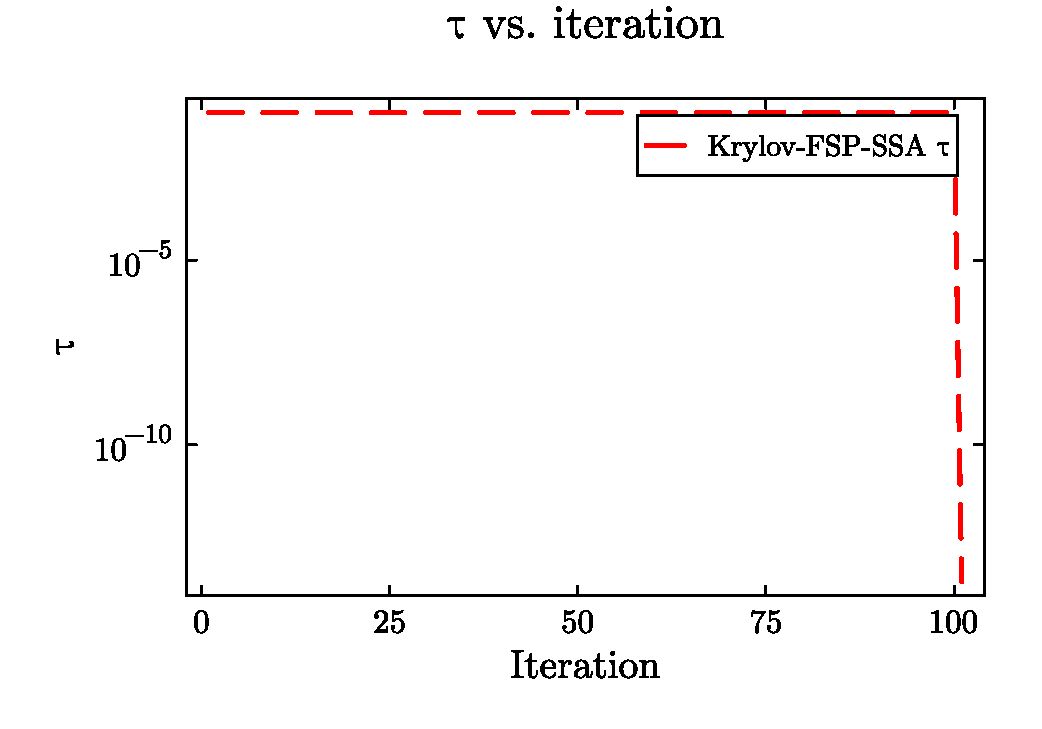
\includegraphics[width=\linewidth]{robertson_comparison.pdf}
    \caption{Robertson system ($t_f = 10^4$): time step vs.\ simulation time (log scale). (a) FP-FSP per-step $\delta t$: non-monotonic, reflecting repeated stochastic autocatalytic burst events. Within each burst cycle $\delta t$ drops sharply as the distribution concentrates, then rises as the burst dissipates. Peak $\delta t \approx 0.026$ during the equilibration phase ($t \gtrsim 3{,}000$). (b) Krylov-FSP-SSA $\tau$ vs.\ iteration: locked in $[3\times10^{-4},\, 3\times10^{-3}]$ by the stiffness of $k_2 = 3\times10^6$, which causes FSP mass-loss violations and numerical overflow in the Krylov matrix exponential for any larger step. The method reaches $t = 227.8$ ($2.3\%$ of $t_f$) in $500$ iterations.}
    \label{fig:robertson_comparison}
\end{figure}

\paragraph{Summary.}
The comparison reveals clearly complementary strengths rooted in different algorithmic choices about step-size control and pruning. On the oscillatory Oregonator, flux-adaptive time stepping provides a decisive advantage: FP-FSP scales $\delta t$ to the instantaneous activity level and maintains a compact state space via flux-based pruning, while Krylov-FSP-SSA is locked at $\tau \approx 10^{-6}$ by mass-conservation failures and cannot complete $t_f = 0.11$. On the bottleneck system, FP-FSP with a fixed step $\delta t = 1/k_2 = 10$\,s keeps the depth-1 expansion pace-matched with the probability wavefront; Krylov-FSP-SSA's exponentially growing $\tau$ produces a 14-state projection that underestimates $\langle C \rangle$ by 40$\times$, with no FSP rejection signal because the missing-row truncation does not reduce $\sum w$ within the truncated system. On Robertson, the stiffness of $k_2 = 3\times10^6$ affects the methods differently. FP-FSP's maximum-flux time step tracks the most active state through repeated autocatalytic burst cycles, with $\delta t$ non-monotonic and peaking at ${\approx}0.026$ during equilibration; FP-FSP completes $t_f = 10^4$ in $662{,}472$ steps ($1{,}117$\,s). Krylov-FSP-SSA with the correct absorbing-form generator is $\tau$-locked by the stiff $k_2$ propensity, reaching only $t = 228$ ($2.3\%$ of $t_f$) in $500$ iterations.

\subsection{Efficiency Under Corrected Krylov-FSP-SSA Parameters}
\label{subsec:corrected_efficiency}

A natural question is whether the efficiency advantages in Tables~\ref{tab:comparison_oregonator}--\ref{tab:comparison_robertson} hold when Krylov-FSP-SSA parameters are tuned to produce \emph{correct} results. Table~\ref{tab:corrected_efficiency} summarises this comparison.

\textbf{Oregonator.} The $\tau$-lock at $\tau \approx 10^{-6}$ arises because the Krylov matrix exponential loses mass conservation for any larger step, owing to the large individual propensities ($k_3 X Z \sim 10^5$). This is independent of $\varepsilon$: tighter pruning reduces $|\mathcal{S}|$ but does not lower the propensity of the surviving states. Krylov-FSP-SSA therefore cannot complete $t_f = 0.11$ at any practical efficiency, regardless of parameter tuning.

\textbf{Bottleneck.} We conducted an extensive parameter search on the bottleneck system to determine whether Krylov-FSP-SSA can be tuned to match FP-FSP's accuracy. The distribution of $C$ given $B{=}1$ is not concentrated at $\langle C \rangle \approx 5$: the bottleneck transition $A \to B$ occurs uniformly over $[0, t_f]$, so $C \mid B{=}1$ spreads approximately uniformly from $0$ to $k_2 t_f = 1000$, with mean $\approx 500$. Accurate resolution therefore requires the projection to track the wavefront at $C \approx k_2 t$ throughout the simulation.

The faithful implementation (Algorithm~2 of~\cite{VoSidje2016}) correctly retains $B{=}1$ via the joint probability-and-derivative filter ($\mathtt{droptol} = 10^{-10}$). The remaining failure is a conflict between step-size growth and state-space expansion. After a successful step, $\tau$ is multiplied by the growth factor (default 2); the $r{=}1$ depth expansion adds only one new $C$-state. For the wavefront to stay within the projection, the expansion depth must satisfy $r \gtrsim k_2 \tau$. As $\tau$ grows (100 $\to$ 3{,}700\,s in the default run), $r$ would need to grow proportionally, making the projection cost scale as the product $k_2 \tau_{\max} \times n_{\mathrm{steps}} \approx k_2 t_f = 1000$. Capping $\tau \leq 1/k_2 = 10$\,s forces $\sim$1{,}000 steps (comparable to FP-FSP) but removes the efficiency advantage of large accepted steps. Increasing $r$ at a fixed $\tau$ improves accuracy but raises per-step cost without addressing the $\tau$-growth coupling.

Empirically, tuning $(\varepsilon, \tau, r)$ over a wide range (Table~\ref{tab:corrected_efficiency}) achieves at best $\langle C \rangle \approx 4.72$ ($\sim$5\% error) at comparable wall time to FP-FSP---which achieves ${<}0.1\%$ error under default parameters. The flux-based method avoids this conflict because FP-FSP uses a fixed step $\delta t = 1/k_2 = 10$\,s, and the exit-flux criterion retains wavefront states regardless of their probability because their outgoing flux $k_2 p(B{=}1, C{=}c)$ is large relative to the total system flux.

\textbf{Robertson ($t_f = 10^4$).} With the correct absorbing-form generator (Algorithm~2 of~\cite{VoSidje2016}), Krylov-FSP-SSA does not complete $t_f = 10^4$. The stiffness of $k_2 = 3\times10^6$ locks $\tau$ in $[3\times10^{-4},\, 3\times10^{-3}]$ via FSP mass-loss violations and numerical overflow in the Krylov matrix exponential at $B{\geq}2$ states; the method reaches only $t = 227.8$ ($2.3\%$) in $500$ iterations ($1.9$\,s). FP-FSP completes $t_f$ in $662{,}472$ steps ($1{,}117$\,s); the maximum-flux time step tracks stochastic burst events, peaking at $\delta t \approx 0.026$. On Robertson, FP-FSP is the only method that completes the simulation.

\begin{table}[!htbp]
\centering
\caption{Efficiency with corrected Krylov-FSP-SSA parameters. ``Default'' uses the parameters from Figures~\ref{fig:oregonator_comparison}--\ref{fig:robertson_comparison}; ``best tuned'' is the best result over a sweep of $(\varepsilon, \tau, r)$ for each system. Best bottleneck result: $\langle C \rangle \approx 4.72$ (${\sim}5\%$ error) at comparable wall time to FP-FSP ($\langle C \rangle = 4.978$, ${<}0.1\%$ error). FP-FSP times from Tables~\ref{tab:comparison_oregonator}--\ref{tab:comparison_bottleneck}.}
\label{tab:corrected_efficiency}
\begin{tabular}{lcccc}
\hline
System & FP-FSP & KrylovFSP (default) & KrylovFSP (best tuned) & Verdict \\
\hline
Oregonator & 33\,s & 74\,s, 2.7\% & DNF ($\tau$-lock, all $\varepsilon$) & FP-FSP wins \\
Bottleneck & 1.0\,s & ${<}0.1$\,s, $\langle C\rangle{=}0.12$ (wavefront trunc.) & 0.9\,s, $\langle C\rangle{\approx}4.72$ (${\sim}5\%$ err) & FP-FSP: ${<}0.1\%$ err \\
Robertson $t_f{=}10^4$ & $1{,}117$\,s, $662$k steps & DNF ($\tau$-lock, absorbing gen.) & DNF (same $\tau$-lock) & FP-FSP wins \\
\hline
\end{tabular}
\end{table}

The key findings reveal qualitatively distinct failure modes. On the Oregonator, the Krylov $\tau$-lock is intrinsic to the mass-conservation criterion and cannot be resolved by any parameter choice: large propensities ($k_3 X Z \sim 10^5$) force $\tau \lesssim 10^{-6}$ regardless of $\varepsilon$. On the bottleneck system, the exponential growth of $\tau$ creates a fundamental conflict with depth-$r$ expansion: keeping the projection pace-matched with the wavefront requires $r \gtrsim k_2 \tau$, but $\tau$ grows without bound; the best achievable accuracy is $\sim$5\% error regardless of $(\varepsilon, \tau, r)$. On Robertson, the stiffness of $k_2 = 3\times10^6$ determines the outcome. With the correct absorbing-form generator (Algorithm~2 of~\cite{VoSidje2016}), Krylov-FSP-SSA is $\tau$-locked at ${\approx}10^{-3}$ and does not complete $t_f = 10^4$; FP-FSP succeeds via maximum-flux time stepping that tracks the stochastic burst structure, completing $t_f$ in $1{,}117$\,s. The overall picture is clear: flux-based methods excel on problems with oscillatory dynamics, connectivity bottlenecks, or stiff bimolecular reactions where the dominant distribution is directly coupled to high-rate transitions; Krylov methods require either a closed-form generator (which masks mass loss at the projection boundary) or a stiff ODE integrator within the Krylov step to handle problems of this type.

\section{Discussion}
\label{sec:discussion}

The numerical results indicate that flux-based pruning can preserve network connectivity across a range of benchmark systems while maintaining competitive compression and accuracy. The comparison with the Krylov-FSP-SSA baseline in Section~\ref{sec:comparison} further demonstrates that the two main contributions---flux-aware pruning and flux-adaptive time stepping---provide complementary robustness advantages on multiscale systems. The method targets two coupled difficulties in adaptive FSP: controlling the loss of important transitions when states are pruned, and selecting time steps that reflect the instantaneous activity level of the system. The flux-based pruning rule protects low-probability states that carry significant probability flow, and the flux-adaptive time-step selection aligns the numerical step size with the dominant rates in the truncated system.

The expansion rule for the proposed method is deliberately simple (fixed $r$-step expansion), and the pruning parameters $(\alpha, \epsilon_{\mathrm{flux}})$ are fixed in time. This suffices for the test problems considered here, but more complicated networks may require additional structure in the adaptation strategy. For example, systems with strong directional drift or localized reaction zones could benefit from combining flux-based criteria with short trajectory bursts \cite{Dinh2016} to identify dynamically relevant regions before committing them to the FSP state space.

The present approach is particularly well suited to mass-conserving systems where the dynamically relevant region remains effectively bounded. Even in that setting, however, flux-aware pruning does not by itself prevent the active set from growing when probability mass is transported over long distances in state space. The bottleneck system in Section~\ref{sec:results} is an example: the distribution is quasi-bimodal, with mass slowly transferring from $(1,0,0)$ to $(0,1,C_{\max}(t))$ along a long chain of intermediate states that carry very low probability but high flux. Our flux-based criterion correctly retains this entire pathway for connectivity, but this also means many “bridge” states must remain active. In such situations, aggregation methods \cite{aggregation,peles,zhang_cao,Cao2016} and conservation-law-based reductions such as slack reactants \cite{slack} provide complementary tools as the intermediate bottleneck states are natural candidates to be lumped into a small number of macro-states while preserving the net flux across the bottleneck. Designing such hybrid schemes and maintaining a transparent error budget in the presence of aggregation remains an interesting problem for future work.


The choice of representation for the generator and the probability vector is another direction for extension. For the moderately sized state spaces in this work ($10^4$–$10^5$ states), Krylov-based exponential integrators \cite{Sidje1998} and sparse matrix representations are sufficient. For higher-dimensional systems, tensor-structured methods \cite{Kazeev2014,Dinh_2020} may be necessary. Extending flux diagnostics and pruning rules to tensor formats would require formulating flux quantities in terms of low-rank factors, which is nontrivial but may be essential for spatial or multicomponent models.

A more structural question is how the adaptive truncation perturbs the long-time behavior of the full chain. In this work we only use conductance and Cheeger-type ideas loosely to motivate flux preservation in Section~\ref{sec:flux-connectivity}, and our analysis focuses on finite-time $\ell^1$ error bounds via flux-based estimates and semigroup contraction. We do not yet track how spectral quantities (such as the spectral gap or mixing time) change as states are added and removed. A natural next step would be to make this connection rigorous by combining conductance bounds with ergodicity-coefficient techniques \cite{rhodius_1993,rhodius_1996} and perturbation bounds for Markov semigroups \cite{pazy_1983}, using flux information to control how much each pruning event can contract the Dobrushin coefficient. This would complement the finite-time, flux-based error analysis developed here by providing spectral stability guarantees for the truncated generators.


From an implementation perspective, several steps of the algorithm can be parallelization. Boundary expansion factorizes over reactions, matrix construction over columns, and Krylov iterations over sparse matrix–vector products. Distributed-memory implementations that partition the state space and communicate flux information along partition boundaries could extend the reach of the method to larger problems without changing the underlying analysis.

Finally, we have focused on time-homogeneous generators. Time-dependent propensities $\alpha_k(x,t)$, arising for example in driven systems or externally controlled networks, fit naturally into the flux-based framework: both the exit rates $w(x,t)$ and the total flux $\Phi_{\mathrm{total}}(t)$ become explicitly time dependent. The same error bounds apply on each step, provided the generator is frozen over that step, and the adaptive step-size rule still responds directly to the changing activity level. A more detailed analysis of time-dependent generators, and of how closely truncated semigroups track the long-time behavior of the full system, would complement the finite-time flux-based error bounds derived here.



\section{Conclusion}
\label{sec:conclusions}

We presented an adaptive FSP method that addresses fundamental challenges in stiff chemical kinetics through flux-based pruning to preserve network connectivity and flux-adaptive time stepping to handle varying activity levels across disparate timescales. The flux-based mechanism identifies and retains low-probability bottleneck states that carry significant flux, preventing catastrophic failures where probability-only truncation severs essential reaction pathways. We derived global error bounds showing that errors accumulate additively due to contraction properties of stochastic generators. Numerical experiments on stiff and metastable benchmark systems demonstrate that the method maintains accuracy with relative errors $\sim$0.01--0.02\% while using state spaces orders of magnitude smaller than exact approaches. A head-to-head comparison with the Krylov-FSP-SSA baseline confirms that flux-aware pruning preserves connectivity on bottleneck systems where probability-only pruning fails, and that flux-adaptive time stepping provides decisive advantages on oscillatory systems with time-varying activity levels. The method successfully handles problems where probability-only pruning fails by removing connector states, though threshold selection requires problem-specific tuning based on system stiffness and timescale separation.


\section{Acknowledgments} We thank the anonymous reviewers for their valuable feedback. The suggestion to examine the bottleneck state example was particularly impactful in clarifying the core motivation for our flux-based approach. The first author also acknowledges Ricky Lee (UC Santa Barbara) for helpful discussions on the mathematical derivations.

\bibliographystyle{siamplain}
\bibliography{references}
\end{document}
